\begin{intro}
  \chapter{Introduction}
  \hyperlink{toc}{Return to TOC}
  \section{\label{ch1:sec0:level1}Preface}
   Few materials possess as great a significance as water. According to the United States Geological Survey, some 71\% of Earth's surface is covered in water\cite{usgswater}. 
   Of this, about 96.5\% is found in oceans, seas, and bays\cite{usgswater}. Adding in contributions from lakes and groundwater, some 97.5\% of water on Earth (about 1.35 
   billion cubic kilometers)\cite{usgswater} is a saline solution which is mainly comprised of Na\sur{+} and Cl\sur{-} with smaller contributions from K\sur{+}, Ca\sur{2+}, 
   Mg\sur{2+}, F\sur{-}, Br\sur{-}, I\sur{-}, and SO\sursous{2-}{4}. While total salinity of these waters varies across the globe, the average salinity of seawater is in the 
   range of 30-35 g/L (or about 500--600 mM, assuming NaCl molar mass)\cite{millero1974physical}. However, there's a case to be made that these simple salts are among those
   few essential materials.
   
   Salts breathe life into our oceans, not just through the organisms which call them home, but also in the stratification of ocean layers based on their salinity which drives
   ocean circulation. This shares an intimate connection with Earth's climate\cite{oceancurrent}. Likewise, salts play a critical role in biology: electrical signalling, regulating 
   pH, stabilizing DNA/RNA, and catalyzing the biological function(s) of hundreds of proteins. The vital role of salts in our diet has similarly steered the course of human 
   history by influencing the location of settlements, trade routes, and sparking human conflicts\cite{multhauf1978neptune}. The chemical properties of salts only became of 
   academic interest in the 1850's\cite{multhauf1978neptune}. Most notable among these early contributors include Arrhenius, Hofmeister, van't Hoff, and Pfeffer. Hofmeister's
   observations made note of the peculiar behavior exhibited by different salts in the precipitation of egg white proteins. It is in conjunction with Arrhenius's theory of 
   electrolytic dissociation that we link these observations to the unique behavior of the component positive and negative charges (ions) comprising the salt. The motion of
   ions powers a great many of our electronic devices allowing us to connect wherever we go with the rest of the world. For a lucky few of us their motion also powers our 
   cars -- and they provide supplemental power and warmth to our real-life Martians: \emph{Spirit}, \emph{Opportunity}, and \emph{Curiosity}\cite{ratnakumar2006li}.
   
   And if we want to keep up with the growing demand for energy in the developing world, batteries and other storage devices will need to evolve to make the ions flow a bit 
   quicker, in greater numbers, and in a greater range of voltages. To do these things, we'll need to develop quantitative and predictive models of ion solvation. This may,
   however, require electronic structure theory to accurately resolve. Since this is a difficult goal, the bar has been set a bit lower to the establishment of a unique, 
   single-ion thermodynamic scale. This, it turns out, is also a difficult problem. However, once this initial goal is solved, it may be possible to translate the physics 
   of advanced modeling into parameter sets for simpler models. The simpler models can help us rationalize ion solvation problems at scales not amenable to interrogation 
   at the electronic structure level.
   
   In this thesis I perform quantum chemical calculations of small alkali/water and halide/water clusters to determine the role that non-electrostatic forces such as dispersion,
   polarization, and charge transfer have on the first solvation shell. In anion/water clusters, these represent about 33\% of the total attractive energetic contributions to
   the interaction energies. Polarization is also essential in the description of cation solvation, while dispersion takes a backseat. My analysis of the charge transfer in 
   these clusters showed that about 20\% of the excess anionic charge spilled out onto the surrounding waters. Charge transfer energies measured with two related methods were 
   found to be inconclusive. These methods are not suitable to ion/water interactions and I make a recommendation of a possibly better method. 
   
   In the second chapter, \emph{ab initio} dynamics is utilized to determine that accuracy is severely compromised when using simple point charge models in simulations of Li\sur{+}/ethylene
   carbonate and Li\sur{+}/propylene carbonate. This is because they lack even a primitive treatment of polarization. Polarization effects are monitored through changes in
   the molecular dipole of solvent molecules distributed near the ion. Relative to the gas phase, the condensed phase dipole moments due to self-polarization are increased by 
   about 30\%, and around 50\% in the first solvation shell of the ion. The close proximity of large dipoles pointing to a common center is believed to create a repulsive 
   contribution that could bring previous single-ion thermodynamic data generated with point charge models into better agreement with experiment.
   
   These initial chapters focus primarily on the interactions between ions and local solvent molecules. This is only part of the puzzle in the determination of a single-ion 
   scale. The other part is a solvent-specific pair of interfacial potentials (one from a distant chemical interface and another from the solvent/ion interface). In a pair 
   of studies, I determine this potential with both contributions using a novel approach to be -0.4 V for water. I argue this potential links two sets of experimental figures 
   for the single-ion solvation properties, a hotly debated topic in the field.
   
   In a follow-up study, I demonstrate that the potential across the solvent/ion interface is present in \emph{all} molecular simulations. It has historically not been taken 
   into account (at least not consistently) by the simulation community and represents a large $\sim$8 kcal/mol error in the hydration free energy of monovalent ions. I relate 
   these findings to the purported solvation asymmetries (differences in these properties for oppositely charged ions) discussed in the literature for different models of
   water, dimethyl sulfoxide, and 1,2-dichloroethane. These solvents cover a wide range of dielectric constants from 10 to $\sim$80. Simulations of divalent ions like
   Mg\sur{2+} and Ca\sur{2+} have always been plagued by poor accuracy and it's possible the huge errors in the free energies of these ions may be in part due to mishandling 
   of the interfacial potential.
   
   This thesis makes several meaningful contributions to the understanding of non-electrostatic forces in ion solvation and proposes a full resolution of a long-standing 
   issue involving the link between two unique scales of single-ion properties derived from experiment. Several indirect experimental results support my finding, though
   there is no conclusive evidence at this time. The surface potential presents several challenges to the force field development community and calls for some standardization 
   of the practice.
   
  \section{\label{ch1:sec1:level1}Hofmeister's puzzle: the specific ion effects}
   The story of the specific ion effects can be traced back to the systematic study of ion effects by Franz Hofmeister (b. 1850, d. 1922), Professor of Pharmacology at the 
   University of Prague, and his students. A series titled, ``Zur Lehre von der Wirkung der Salze'' which translates to ``About the science of the effect of salts'' recounts
   the findings of several publications. The original document in German is available at Ref. \cite{hofmeister1888lehre} and an English translation provided by Werner Kunz
   et al. in Ref. \cite{kunz2004translation}. A short biography of Professor Hofmeister can be found at Ref. \cite{abernethy1967franz}.
   
   Though the scope and importance of his work has been likened to that of Mendel to genetics\cite{kunz2004translation} (and also not -- Ref. \cite{jungwirth2014beyond}), 
   Hofmeister was a proficient and interdisciplinary researcher as pharmacy tied together the fields of chemistry, physiology, and botany\cite{abernethy1967franz}. His work 
   properly identified lactose as the sugar central to the condition known as lactosuria (formerly, glucosuria) common in pregnant women and newborns\cite{abernethy1967franz}. 
   He published on vitamin deficiencies as well and made notable contributions to coordination chemistry and separations\cite{abernethy1967franz}. Altogether, Hofmeister and 
   his students published about 400 papers\cite{abernethy1967franz}. And yet, this thesis concerns the lingering questions resulting from a handful of these articles. However, 
   the challenge to address his observations, often called the Hofmeister or specific ion effects, from a theoretical perspective, has remained one of the greatest in the field 
   of physical chemistry since.
   
   \subsection{\label{ch1:sec1:level2}The Hofmeister series}
    Lewith and Hofmeister's seminal work on the specific ion effects established the relative cationic and separate anionic effects on ``precipitating action, dissolving action, 
    and lyotropic swelling of proteins along with diarrhetic action, diuretic action, water binding, osmotic pressure, and other physical chemical phenomena''\cite{abernethy1967franz}.
    By holding the cation constant, the anion effect could be isolated and ordered in a series reflecting the concentration required to, for example, precipitate the hen egg white
    proteins (predominantly globulins and albumins). In order of decreasing effectiveness,
    
    \begin{equation}\label{hof1}
     \begin{split}
     \text{CO}\sursous{2-}{3} > \text{SO}\sursous{2-}{4} > \text{HPO}\sursous{2-}{4} > \text{OH}^{-} > \text{F}^{-} >~&\text{CH}\sous{3}\text{COO}^{-} > \text{Cl}^{-} \\
                              &> \text{Br}^{-} > \text{NO}\sursous{-}{3} > \text{I}^{-} > \text{ClO}\sursous{-}{4} > \text{SCN}^{-},
     \end{split}
    \end{equation}
    
    \noindent with a complementary series for cations as well,
    
    \begin{equation}\label{hof2}
     \begin{split}
     \text{C}(\text{NH}_{2})_{3}^{+} >> \text{Ca}^{2+} > \text{Mg}^{2+} > \text{NH}_{4}^{+} > \text{Li}^{+} > \text{Cs}^{+} \approx \text{Rb}^{+} >~&\text{Na}^{+} > \text{K}^{+} \\
     &> \text{N}(\text{CH}_{3})_{4}^{+} > \text{TEA}^{+},
     \end{split}
    \end{equation}
    
    \noindent where TEA\sur{+} is tetraethylammonium and C(NH\sous{2})\sursous{+}{3} is guanidinium. I've chosen the ordering presented in Ref. \cite{mazzini2016specific} which
    is most consistent with the spirit of the series Hofmeister inspired\cite{kunz2004translation}. This series is presented in other forms as well, not all of which are logically
    consistent with the results of Hofmeister (or with each other, for that matter), see Refs. \cite{collins2004ions,kunz2010book,marcus2009effect,salis2014models,schwierz2016reversed}. 
    Discrepancies primarily occur within the cation series which is not as well-established as the anion one. This is because the affect on protein solubility and many other properties
    are dominated by the anion\cite{hamaguchi1962effect,marcus2009effect}. In fact, Table 1 in Hamaguchi et al. is a wonderful example of the minimal impact cations tend to have, in 
    this case on the denaturation of sea urchin DNA in 4 M salt solutions\cite{hamaguchi1962effect}. The cation trend also has some non-obvious placements (e.g., Cs\sur{+} and Rb\sur{+} 
    between Li\sur{+} and Na\sur{+}), with a terrific illustration of the variance in the literature presented in Ref. \cite{mazzini2016specific}. To explore this further, I found it 
    instructive to revisit this data expressed in grams of salt added per 100 mL of solution and convert the grams of sulfate salts to moles of the respective cations. Using the results 
    as published in Ref. \cite{kunz2004translation}, the ordering is just as published above in Eq. \ref{hof2} with 0.1323 moles of Mg\sur{+}, 0.1566 moles of Li\sur{+}, and 0.1604 moles 
    of Na\sur{+} present. This ordering differs from that if just ordering the ions based on the mass of the salt or even moles of the whole salts required. This ambiguity greatly 
    undermines the utility of the series and serves mainly as a source of confusion and frustration.
    
    The trends above are also denoted as the \emph{direct} Hofmeister series. There are a number of examples of cases where the inverse series is observed instead, called the
    \emph{reverse} Hofmeister series, a few of which are summarized in Refs. \cite{heyda2010reversal,parsons2009direct,schwierz2016reversed}. The reverse series is also observed at pH
    below the isoelectric point of a protein\cite{salis2014models}. Later I'll discuss a less ambiguous partitioning of ionic behavior based on the ion hydration entropies.
    
    Putting aside these details, the interesting thing about Hofmeister's observations is that they link both salt \emph{concentration} and \emph{composition} to the behavior of 
    other solutes in solution. The former is the more obvious: the solubility of various salts in water and other polar solvents is often exceedingly high, but finite all the same 
    through the activity coefficient\cite{burgess1978metal}. The compositional dependence of many of these properties is perhaps less obvious but is pervasive throughout chemical
    literature. Several examples of specific ion effects in both aqueous and non-aqueous media are listed below,
    
    \begin{itemize}
        \item activity coefficient\cite{xie2013simple},
        \item surface tension increments\cite{bostrom2001surface,marcus2016surftension,pegram2007hofmeister,slavchov2012surface},
        \item freezing point depression, osmotic pressure, vapor pressure\cite{franks2000water},
        \item solvent viscosity\cite{collins2004ions}, 
        \item surface potential increments\cite{marcus2016surftension} (ion concentration changes the quantity discussed in Chapter \ref{ch1:sec4:level1}, but these are relative
        shifts and so do not necessarily justify a particular value of the air/water surface potential, but does rather significantly perturb pH measurements via glass 
        electrodes\cite{bostrom2003hofmeister}), 
        \item selective adsorption of ions to chemical interfaces\cite{carrier2016ionsatowinterface,conboy1997shg_tatb,ben2016interfaces,jungwirth2002airwat,jungwirth2006airwat,luo2015electrobreak,ou2016molecular,pratt1992contact},
        \item isoelectric point of the air/water interface\cite{beattie2009basic,beattie2014surfacid,buch2007surfacid,mishra2012surfacid,vacha2007autoionization},
        \item brine rejection stratifying deep ocean waters which act as reservoirs of dissolved CO\sous{2}\cite{shcherbina2003direct,vrbka2005brine} and lead to the formation of 
        brinicles\cite{frozenplanet,martin1974ice},
        \item double-layer forces\cite{bostrom2003hofmeister,ruckenstein2014specific}, 
        \item morphological and rheological properties of dipeptide-based hydrogel\cite{roy2012dramatic},
        \item clouding point temperature\cite{cremer2009lysozyme}, 
        \item kinetics of amyloid formation, especially at low ionic strength\cite{marek2012ionic}
        \item lower critical solution temperature\cite{zhang2005specific}, 
        \item CO\sous{2} capture by nanoporous materials\cite{shi2016co2capture},
        \item bubble coalescence (see excellent study in Ref. \cite{craig1993effect} and review in Ref. \cite{craig2004bubble}),
        \item frother stability used in foam floatation extraction particularly in separating heavy metals from wastewater and ore extraction\cite{ozdemir2013specific}
        \item apparent surface charge of oil and air bubbles suspended in water, electrophoretic mobility (see recent survey in Ref. \cite{zimmermann2010hydroxide} with an alternative
        contribution discussed in Ref. \cite{rick2012bubbles}; $\zeta$-potential is too small though, so it's a less likely explanation)
        \item electrophoretic mobility of bare magnetite nanoparticles\cite{vereda2015specific},
        \item ion channel activity\cite{asthagiri2010ion,chen2016free,dreyer2013role,guidoni1999potassium,guidoni2000water,guidoni2002tetraethylammonium,liu2013equilibrium,roux2011ion,zhang2012water},
        \item muscle contraction and neuronal signalling\cite{purves2001neuroscience,szent1975calcium},
        \item enzyme activity\cite{cacace1997hofmeister},
        \item macromolecule (i.e., protein, DNA, RNA, surfactant) stability and
        solubility\cite{abernethy1967franz,cacace1997hofmeister,collins1995,collins2004ions,collins2007review,kunz2004translation,kunz2010book,marcus2009effect}.
    \end{itemize}
    
    An even more extensive list complete with additional references, albeit a bit dated, can be found in Ref. \cite{collins1985hofmeister}. In each of these examples 
    the chemistry and concentration dependence of these effects are difficult, if not impossible, to separate above very dilute conditions. A reasonable cutoff is on the order
    of the millimolar (mM) scale. The specific behavior of salts discussed above has profound implications in fields as diverse as soil\cite{yu2016soil},
    marine\cite{jungwirth2006airwat} and 
    atmospheric\cite{baer2014investigation,buch2007surfacid,galib2014oceanacid,galib2014hbondingcarbonic,jungwirth2002airwat,jungwirth2006airwat,lewis2011does} chemistry, 
    climate modeling, physiology, industrial chemistry especially transport of raw ingredients\cite{hodson2013personal}, electrochemistry, energy storage devices\cite{ayse2016ecpc},
    chemistry in mixed solvents (e.g., in liquid chromatography columns)\cite{suu2015mixedpH}, synthesis with charged intermediates, polymer self-assembly\cite{roy2012dramatic}, and 
    beyond. 
    
    Unsurprisingly these fields routinely deal with mM and greater concentrations of salts, motivating the need for continued efforts such as my own to develop a quantitative
    model of these effects. It can be difficult to know where to start however. Fortunately we can draw inspiration from other life experiences and so first work towards solving the 
    simplest case: that of ion solvation in water\cite{duignan2014ion}. The target here is the accurate determination of single-ion solvation properties and especially the solvation
    free energy from simulation\cite{hunenberger2011sp}. The desired theoretical model should take care to accommodate the major contributions to the free energy change, 1)
    interaction part between the ion and solvent as well as 2) a change in the free energy associated with the reorganization of solvent molecules around the ion (cavity formation).
    The interaction part can be split up into 1a) local effects arising from the strong $\approx$ 1 V/\AA~fields around the ions\cite{sellner2013ionfield} and 1b) distant solvation 
    effects which may be amenable to computationally inexpensive approximations in dilute conditions, and 1c) interactions with a distant surface or chemical interface. 
    
    A focus on simulations of ion-ion interactions was common in the late 1980's and early 1990's and has experienced a recent resurgence in interest with publications by Duignan et
    al.\cite{duignan2014ion}, Luo et al.\cite{luo2013simulation}, Lund et al.\cite{lund2009dielectric}, Fennell et al.\cite{fennell2009ion}, Shi and Beck\cite{shi2017lmwa}, and others. 
    Activities are of critical importance to these effects as well and there is no ion activity more ubiquitous to science than that of the proton H\sur{+}.
    The definition of pH is only nominal as it depends explicitly on the proton activity (pH=-log $\alpha\sous{H\sur{+}}$), which is not directly measurable by 
    experiment\cite{guggenheim28,iupac,rockwood2015meaning}. This is also a big topic among researchers studying ocean acidification trends where an uncertainty of 0.003 pH units
    is desired to facilitate better comparison with decades worth of acidity data\cite{cao2015considerations,dickson1993measurement,dickson2015metrological}. While many of the 
    models used are predicted to struggle at moderate to high salt concentration, they are still useful for surveying the plausibility of a recent qualitative development for 
    rationalizing the Hofmeister effects called the Law of Matching Water Affinities which I discuss below.
     
   \subsection{\label{ch1:sec1:level3}The language of ion solvation: kosmotropes and chaotropes}
    Though the ion solvation community has the main aim of developing a quantitative theory of the specific ion effects, it is instructive to review some of the recent attempts to
    discern the contributing factors to the Hofmeister series and conceptualize the differences between the ions. This exercise makes the connection between a numerical model and 
    the single-ion solvation thermodynamic scale more apparent.
     
    In the series presented in Eqs. \ref{hof1} and \ref{hof2}, the ions are ranked by their ability to precipitate egg white proteins with the molar concentration of the salt 
    required increasing from left (most effective) to right (least effective). Precipitating proteins with salt is known as ``salting-out.'' Salts composed of ions on the left side
    of the series above do this effectively and promote protein-protein interactions which form aggregates that are less soluble in water. The anions in good precipitating salts 
    are typically strongly hydrated\cite{collins2004ions}. Salts composed of ions on the right side of the series destabilize protein-protein interactions and initially increase 
    their solubility (``salt-in'') and so require greater concentrations to precipitate the proteins. This property is known as chaotropicity and was initially interpreted as an 
    entropic effect related to the ``disorder'' in proteins, lipids, DNA, RNA, and other macromolecules induced by the ions in solution\cite{abernethy1967franz,ball2015water,hamaguchi1962effect}. 
    Collins et al. and others argue that the cation trend should be the reverse of that displayed in Eq. \ref{hof2} because the divalent ions interact with amide and other polar 
    functional groups on the protein surface and enhance the solubility, see Ref. \cite{collins2004ions} and the related references therein (10, 53, 86-89). In Ref. 88 of that
    paper, the authors note that solution pH affects the divalent (several) results but not the monovalent ion results (Na\sur{+})\cite{arakawa1984mechanism}. It's complicating
    factors like this which steer us from the original spirit of the Hofmeister series towards something a bit more palatable. 

    The work of von Klobusitzsky established that the placement of anions in the Hofmeister sequence could be modified by changing the complementary cation, as in the example
    also summarized in Ref. \cite{abernethy1967franz}. Collins\cite{collins1985hofmeister,collins1995,collins2004ions,collins2007review} and Arakawa\cite{arakawa1984mechanism} also
    discuss a competition for waters among protein-solvating cations and anions and this interpretation is visited in Refs. \cite{ball2015water,marcus2009effect}. These findings 
    promote a connection between the Hofmeister series and the relative ability of the ions to compete with each other and other solutes for solvating waters. This has led researchers
    to study the local solvation structure around the ions and ascribing the controversial tags of water `structure-maker' and `structure-breaker' to them. These terms apparently 
    correlate with the ability of the solute (not necessarily ionic) to increase the order of waters around it (structure-maker, kosmotrope) or decrease their order (structure-breaker, 
    chaotrope). 
    
    The difference between chaotrope used here and used above is the subject of much debate\cite{ball2015water,marcus2009effect}, with Marcus stating the terms are more or less 
    equivalent in this context. Much like the difficulties in deriving a consistent cation Hofmeister series above, the distinction between an ordering and disordering ion is 
    difficult to make given that ion effects are localized within the first or second hydration 
    shell\cite{collins2007review,williams2012nanodrops,jungwirth2013hofmeister,jungwirth2014beyond,ninham2011review,saha2016impact}. 
    Effects on water hydrogen bonding patterning are limited to about 1 nm even for di- and trivalent ions\cite{williams2012nanodrops,williams2015trivalent,williams2015crystal}. 
    
    The length scale of ionic forces in solution is itself a \emph{kind of} debate, see Ref. \cite{ninham2011review} where long-ranged ionic forces are termed (probably jokingly)
    as `heretical' and Ref. \cite{chen2016electrolytes} which claims monovalent ions have a measurable effect at a range of over 20 nanometers. Keep in mind, the Bjerrum length in 
    water (dielectric constant of 78) is about 7 \AA, beyond which the Coulombic attraction is smaller than the thermal energy at room temperature. You be the judge of that.
     
    As the tags of structure-making/breaking fell from favor, the nomenclature evolved to reflect differences in surface charge density and the relative strength of the ion/solvent 
    to solvent/solvent interactions instead. In this context, a kosmotrope is a small ion with high surface charge density (think \emph{hard ion} from hard-soft acid-base theory) which
    are strongly hydrated and chaotropes are weakly hydrated with low surface charge density. The ordering makes significantly more sense (cutting it down to just the alkali-halide
    series) and is strongly tied to the strength of hydration forces,
    
    \begin{equation}\label{hof3}
     \begin{split}
     \text{F}^{-} > \text{Cl}^{-} > \text{Br}^{-} > \text{I}^{-},
     \end{split}
    \end{equation}
    
    \noindent and the cation series,
    
    \begin{equation}\label{hof4}
     \begin{split}
      \text{Li}^{+} > \text{Na}^{+} > \text{K}^{+} > \text{Rb}^{+} > \text{Cs}^{+}.
     \end{split}
    \end{equation}
    
    \noindent Though, and rather confusingly, all three versions are still in use (and sometimes interchangeably, \emph{because why not make it difficult?})\cite{ball2015water}.
    
    But what does it mean to be strongly hydrated? Weakly hydrated? Are there any properties that can quantify this distinction?
    
    Collins et al.\cite{collins2007review} relate the kosmotrope and chaotrope distinction to the sign of the Jones-Dole B coefficients taken from the Jones-Dole viscosity 
    relation. This series quantifies the relative change in solution viscosity upon the addition of electrolytes. It is a series expansion of the form, $\eta$/$\eta\sous{0}$ 
    = 1 + A$\sqrt{c}$ + Bc + Dc\sur{2}, where $\eta$ is the salt solution viscosity, $\eta\sous{0}$ the viscosity of the pure solvent, c the salt concentration, and A, B, and D
    are fitted parameters. The B coefficient is typically interpreted to reflect the strength of ion/solvent interactions\cite{jenkins1995viscosity}. The water/water interaction
    is assigned a value of 0. Ion/solvent interactions stronger than water/water give B $>$ 0 and those weaker B $<$ 0. The alkali/halide series match up exceptionally well 
    with the B-coefficients. Na\sur{+} (0.086) and Cl\sur{-} (-0.007) sit very near the 0 mark, with Na\sur{+} considered a weak/borderline kosmotrope and Cl\sur{-} considered 
    a weak/borderline chaotrope. These data can be found in the previous Collins review in Ref. \cite{collins2004ions}. 
    
    Assuming the B coefficient to track temperature and pressure behavior of the komso/chaotropic nature of the ion, then Li\sur{+} and F\sur{-} become less kosmotropic while 
    all the others see increases in their B-coefficients from 0--$\SI{55}{\degreeCelsius}$\cite{jenkins1995viscosity}. Oparin et al. reach similar conclusions for LiCl, NaCl, 
    and KCl electrolytes\cite{oparin2002relationship}. They also find that under extreme pressures, Na\sur{+} becomes chaotropic\cite{oparin2002relationship}.
    
    In brief, the trend is inconsistent for polyatomic ions. My favorite example of this is the ammonium, tetramethylammonium (TMA), and tetraethylammonium (TEA) series where
    the B coefficients increase along the series (Table 5 in Ref. \cite{jenkins1995viscosity}) but these ions are actually becoming softer (increasing radius) and more weakly 
    hydrated (TMA bulk hydration free energy $\mu\sursous{ex}{b}$ is -48 kcal/mol and TEA $\mu\sursous{ex}{b}$ is -41 kcal/mol)\cite{abraham1978}. Ammonium data is not available 
    in this paper, but take a look at Ref. \cite{marcus1985book} to get an idea of the difference in $\mu\sursous{ex}{b}$ between ammonium and TMA (TEA $\mu\sursous{ex}{b}$ is 
    set to zero in this data).
    
    Another common metric used to distinguish the kosmotropic and chaotropic scale is the entropy of locally coordinated water molecules. An experimental quantity is discussed
    in Ref. \cite{collins2007review} (Figure 5) and in more detail in Ref. \cite{collins1985hofmeister} (Figure 3) (it's a reproduction from an old book, which itself is a 
    reproduction from an even older paper). The original authors measured the entropy change relative to bulk water for a water adjacent to each of the alkali/halide ions, 
    assuming the ion solvation effect propagated no further than the first hydration shell. The quantity plotted is the bulk entropy minus the first shell entropy which 
    is negative for \emph{all} chaotropes (K\sur{+}, Rb\sur{+}, Cs\sur{+}, Cl\sur{-}, Br\sur{-}, and I\sur{-}). The interpretation here is that these ions only weakly 
    associate with the water and liberate the bound water from the bulk. This is synonymous with the `structure-breaker' term discussed previously (but importantly, the 
    ions don't structure waters over a great distance). \emph{Waters} bound to Li\sur{+} and F\sur{-} are less mobile than those in the bulk. Again, the localized nature of 
    these effects makes moot the idea of long-range structuring of water by the ions. Collins et al. also discuss the signatures of chaotrope and kosmotrope influence through
    proton nuclear magnetic longitudinal reorientational times\cite{collins1985hofmeister}. Waters situated around chaotropes tend to `tumble' faster than bulk waters, while those
    around kosmotropes `tumble' slower.
    
    The translational and rotational components of the entropy of distinguished water molecules has also been recently explored using molecular dynamics 
    simulation\cite{saha2016impact}. Each component was reduced relative to these same quantities in bulk water, with about 80\% of the effect captured in the first shell, 
    consistent with the assumptions made above, and about 20\% of the effect arising from the second hydration shell. Cations reduced both the translational and rotational 
    entropies of first shell waters by nearly equal amounts, while monoatomic anions reduced the rotational entropy by a few multiples over the translational entropy. 
    This is not observed with polyatomic anions possibly due to the greater number of binding sites (anions were SO\sursous{2-}{4} and ClO\sursous{-}{4}). The author finds
    an approximately linear relationship between the reduction in the distinguished water translational entropy and surface charge density.
    
    Finally, Beck used molecular dynamics and a free energy partitioning scheme called the local molecular field theory (with temperature derivatives) to compute spatially
    separable components of the solvation entropy of the alkali/halide ions\cite{beck2011lmft,beck2011local}. Spatial conditioning is applied to the electrostatic contribution,
    which divides into a local and far-field (distant) part. The author finds that kosmotropic ions give an ion specific, sizable, and negative s\sursous{ex}{loc}, which 
    is the local part of the electrostatic contribution to the hydration entropy. Beck likewise found chaotropes to give positive s\sursous{ex}{loc}, with a small 0.5 cal/mol-K 
    contribution for Cl\sur{-}, solidifying its reputation as a borderline chaotrope. In Figure 2 of Ref. \cite{beck2011local}, the author plots this entropic term versus the
    inverse of the ion size. The anion trend line is approximately linear with a large slope while the cation line (albeit of only two data points) is much flatter, implying  
    less specificity between the ions considered. This perfectly mirrors the conclusions of Marcus and Hamaguchi et al. mentioned in a previous 
    section\cite{hamaguchi1962effect,marcus2009effect}.

    Three of these properties are related explicitly to solvation entropies for either the coordinated water molecule(s) or the single-ion quantity itself. The B-coefficients
    may also be related to the partial molar entropy of solvation as well, interestingly enough\cite{nightingale1959phenomenological}. Entropic quantities also aren't as 
    significantly impacted by sign-dependent surface potential effects either, which is a bonus. In my opinion, these examples serve to illustrate the connection between a 
    quantitative model of the specific ion effects and single-ion solvation thermodynamic properties. We must pursue the latter in order to develop the former. 
    
    Additionally, authors like Evens et al.\cite{evens2008hofmeister} have demonstrated that the simple ranking of ions based on their main effect is of limited use because
    1) the one-dimensional ranking of ions gives little to no insight on the nature of ion/solvent, ion/solute (protein, DNA, etc.), or ion/ion interactions 2) the ordering
    depends on solution temperature, pressure, possibly on solution pH, electrolyte concentration, protein concentration, the amount of dissolved gases, begging the question
    what the ordering for a particular set of conditions is all that useful for, and 3) it's rare in practical applications that only a single salt species is present in
    solution. Nevertheless, these series are essential. They are placeholders for a deeper understanding and spring up when we observe salt specific behavior we can't quite 
    wrap our heads around. That's useful in its own right.
    
   \subsection{\label{ch1:sec1:level4}The law of matching water affinities}
    A kosmotropic ion is said to be strongly hydrated while a chaotropic ion is said to be only weakly hydrated. Collins linked these observations to complex Hofmeister behavior 
    on the basis that ions of opposite charge form contact ion pairs spontaneously only when they have similar water affinities (the familiar \emph{`like' seeks `like'} 
    trope)\cite{collins2004ions,collins2007review}. Unmatched ions dissolve because the larger ion screens the smaller one in strongly polar solvents\cite{lund2009dielectric}.
    The general concept is very similar to the Pearson hard soft acid base theory\cite{pearsonhsab0,pearsonhsab1,pearsonhsab2}.
    
    This means that kosmotrope-kosmotrope and chaotrope-chaotrope pairs are preferred to the solvent separated (i.e., dissolved) species, forming contact ion pairs which partially
    or entirely exclude the solvent between them. These pairs are marked as having a positive heat of solution with the individual ions having similar heats of hydration and so 
    are not very soluble. This is best illustrated in the volcano plot of Collins et al. reproduced in Figure \ref{fig:collinsvolcano}\cite{collins2007review}. Crystalline salts 
    comprised of mixed pairs of chaotrope-kosmotrope and kosmotrope-chaotrope (cation-anion) ions release heat upon being placed in solution (and so dissolve) and form the slopes
    of the volcano where the anion is better hydrated on the left slope and the cation better hydrated on the right slope.
    
    This characterization has proven successful already in untangling the mystery behind these effects in many experiments which are reviewed in Refs. \cite{collins2004ions} and
    \cite{collins2007review}. I mentioned this before, but this keen observation has motivated a renewed interest in simulating ion/ion interactions between matched and unmatched
    pairs to verify the method at least theoretically and try to understand some of the driving forces selecting the dissolved or solvent-excluded states. My colleague Yu Shi 
    published a paper on the results he obtained applying the local molecular field theory I discussed to the free energy profiles (potential of mean force, pmf) of matched and 
    unmatched alkali/halide salts as they approach each other\cite{shi2017lmwa}. This has been done before (see references mentioned above and a recent study by Baer et 
    al.\cite{baer2016local}). The pmf of the solvent-excluded state has a free energy minimum where the ions are very close to each other and the solvent-separated pair have a 
    minimum at a greater distance which is spaced enough to allow waters to bridge the ions, see Ref. \cite{fennell2009ion} for terrific illustrations. But no one else has been 
    able to partition the pmf into contributions made from particular interactions. This is the subject of the rest of the opening chapter. We know there's specificity, we know 
    hydration forces (ion/solvent interactions) are involved, but now we ask,
    
    \begin{itemize}
        \item What sort of interactions? 
        \item How strong are they relative to one another?
        \item Do we need electronic structure theory to solve everything?
        \item Will a simpler model work far away from the ion? 
        \item Do chemical interfaces contribute to single-ion thermodynamics? 
        \item If so, what is the contribution?
        \item How can we compare our simulation results to experiment?
    \end{itemize}
     
    These are all questions I address in the following sections and in the following chapters where I discuss my own work. 
     
\begin{figure}
 \begin{center}
  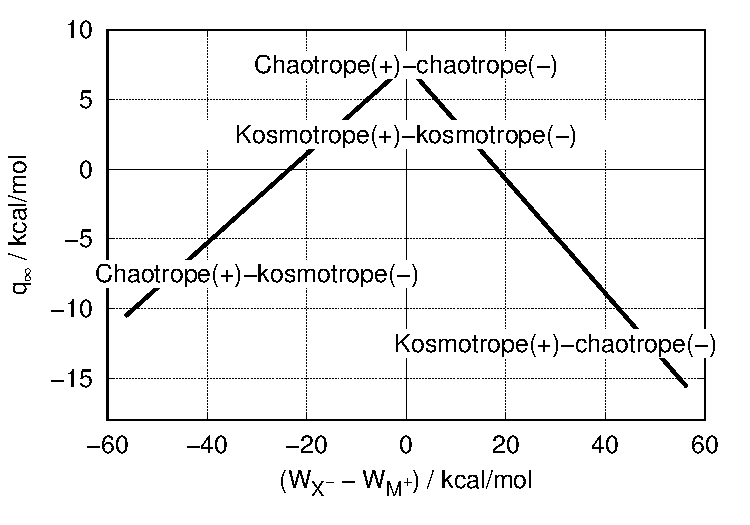
\includegraphics[width=0.98\linewidth]{images/volcano_collins.pdf}
 \end{center}
 \caption[Collins' volcano plot to distinguish similar and dissimilar ion pairs]{\label{fig:collinsvolcano}Ions can be classified as chaotropes (weakly hydrated) or
 kosmotropes (strongly hydrated). This plot illustrates the relationship between the standard heat of solution (at infinite dilution) of crystalline alkali/halide salts and 
 the difference between the absolute heats of hydration of the respective ions. The degree of similarity or dissimilarity between the ions comprising a salt can be qualitatively 
 assessed from its placement into one of four distinct regions (labelled above). Figure recreated from Ref. \cite{collins2007review} (\textcopyright Elsevier Biophysical Chemistry, 
 reprinted with permission) in order to enhance image clarity.}
\end{figure}    

  \section{\label{ch1:sec2:level1}Models of ion solvation}
   Modeling is one of the most effective tools in scientific research. Models unify results, rationalize observations, and grant some level of predictive power under unexplored
   conditions. In this section I briefly review several important advancements in the development of numerical models of the ion solvation problem. 
   
   As discussed above, all of these methods target analytical or numerical solutions to several target properties of the simple ion-into-water scenario: 1) solvation free energies, 
   enthalpies, and entropies of individual ions at infinite dilution, 2) activities and osmotic coefficients, and 3) surface tension increments. Each of these methods make assumptions
   on the nature of ion/solvent and ion/ion interactions. Their shortcomings help us address issues with the underlying physics and so have been instrumental in the evolution of 
   such models over the last century. 
   
   The methods discussed here also share the treatment of solvent as a mathematical continuum in common, meaning no ball-and-stick molecular models are required except for the ion 
   itself. The earliest models covered here ignore the solvent reorientational contributions to the free energy and assume the ion/solvent interactions to be purely electrostatic. 
   Successes and failures of these models will be discussed.
   
   In the second section, I'll explore the corrections considered in modern continuum solvation models. The corrections consider the role of several additional ion and solvent 
   properties which are believed to impart ion specific behavior: dispersion interactions, polarization, charge transfer, cavitation energy (solvophobic effect), ion size (charge 
   density), and surface potentials across chemical interfaces. Extra attention will be paid to the model of Duignan et al. which I believe, despite my criticisms levied against
   it throughout this thesis, is an exceedingly simple and elegant theory of ion solvation. The model is capable of handling ions in dilute solutions, ions moving towards the 
   air/water interface (this is the primary area of disagreement), and ion/ion interactions. 
  
   \subsection{\label{ch1:sec2:level2}The early models}
    Probably the most familiar of these models is the Debye-H\"{u}ckel theory. Debye-H\"{u}ckel theory assumes the interactions between ions to be purely electrostatic (which is
    rigorously true, see the Hellmann-Feynman theorem\cite{politzer2015mathematical}). The solvent is modeled as a dielectric continuum through the dielectric constant and the 
    ion charge density with a Boltzmann distribution. It is only \emph{valid} in the limiting case of low concentrations (<100 mM).
    
%    The starting point for this theory is the Poisson relation,
    
%    \begin{equation}
%        \nabla^{2}\psi(r) = -\frac{\rho(r)}{\epsilon}
%    \end{equation}
    
%    \noindent which defines an electrostatic field $\psi(r)$ due to the charge density $\rho(r)$ in a dielectric medium. The charge density in the Debye-H\"{u}ckel
%    theory is chosen as a Boltzmann distribution,
    
%    \begin{equation}
%        \rho(r) = q_{i}c_{i}^{\infty}\lambda(r)\cdot\exp\left(-\frac{q_{i}\psi(r)}{k_{B}T}\right)
%    \end{equation}
    
%    \noindent where c$_{i}^{\infty}$ is the bulk charge density of an ion with charge q$_{i}$, and $\lambda(r)$ denotes the accessibility of an ion to position $r$ 
%    (typically set to 1, so ignored hereafter). Combining these expressions leads to the Poisson-Boltzmann relation for a collection of charges,
    
%    \begin{equation}
%        \nabla^{2}\psi(r) = -\frac{1}{\epsilon}\sum_{i}c_{i}^{\infty}q_{i}\cdot\exp\left(\frac{q_{i}\psi(r)}{k_{B}T}\right).
%    \end{equation}
 
%    \noindent A position dependent dielectric can be substituted into the expression above as well to mimic chemical interfaces. The equation above is an exact relation for 
%    describing the field of a charge distribution and though solvers do exist, they are typically far slower than other approximate methods.
    
%    Debye and H\"{u}ckel worked out a solution for the electrostatic potential experienced by a spherically symmetric ion \emph{j} suspended in a dielectric medium 
%    for $r$ less than $\alpha$, where $\alpha$ traces the ion surface.
    
%    \begin{equation}
%        \psi(r)_{j} = -\sum_{i}\frac{q_{i}\kappa}{\epsilon\left(1+\kappa\alpha\right)}
%    \end{equation}
    
%    \noindent where $\kappa$ is the inverse Debye length, $\kappa = \sum_{i}\sqrt{\frac{4\pi q_{i}^{2}c_{i}^{\infty}}{k_{B}T\epsilon}}$. The negative of the result of taking
%    half the potential multiplying the charge of ion \emph{j} gives us the excess chemical potential $\mu^{ex}_{j}$. Setting the two sides of the equation equal to one another 
%    and rearranging to solve for $\ln\lambda_{j}$ defines the activity coefficient. Converting from the molar to molal scale allows ionic strengths to be described from this 
%    result as well. Ionic strength can also be expressed in the molar scale, but because the volume change for higher ionic strengths is not strictly additive, it is preferable
%    to use the molal scale in practice.
    
%    The electronic part of the solvation free energy can be derived by substituting the potential above into the Debye charging expression or by solving the integral G = 
%    $\int \frac{U_{e}}{T^{2}} dT$ where $U_{e,j}$ is the electronic potential energy of ion \emph{j} in the field of all the other ions. The equation used in the original
%    paper\cite{debye1923theorie} neglects pressure-volume work under the assumption that the solvent is incompressible.
    
    Debye and H\"{u}ckel expressed the low concentration limit of the free energy of an ion ($\mu_{i}$) in this field as
    
    \begin{equation}
        \mu_{i} = k_{B}T\ln\Lambda_{i}^{3} + k_{B}T\ln c_{i} - \frac{\kappa q_{i}^{2}}{2\epsilon}
    \end{equation}
    
    \noindent where $\lambda$ is the de Broglie thermal wavelength, c\sous{i} the concentration, and the third term is the electrostatic part of the free energy,
    making use of $\kappa^{2} = \frac{4\pi}{\epsilon k_{B}T}\sum_{i}q_{i}^{2}c_{i}$, where $\kappa^{-1}$ is the inverse Debye length. This equation can be rewritten as
    
    \begin{equation}
        \mu_{i} = k_{B}T\ln\Lambda_{i}^{3} + k_{B}T\ln c_{i} + k_{B}T\ln\gamma_{i}
    \end{equation}
    
    \noindent where $\ln\gamma_{i} = -\frac{\kappa q_{i}^{2}}{2\epsilon k_{B}T}$ is the activity coefficient of the i\emph{th} ionic species. This is not accessible to 
    experiment, so the mean activity coefficient is measured instead, giving $\ln\gamma_{\pm} = -\left|q_{+}q_{-}\right|\frac{\kappa}{2\epsilon k_{B}T}$. A plot of the
    $\ln\gamma_{\pm}$ versus $\sqrt{I}$ is linear at low concentrations, where I = $\frac{1}{2}\sum_{i}q_{i}^{2}c_{i}$ and is the (typically) molal ionic strength. That
    is, the approximation of ion-ion interactions as essentially non-interacting, screened point charges is reasonably accurate for low concentrations. At higher 
    concentrations, the limiting expressions break down and exhibit significant deviation from experiment. Application of the Debye-H\"{u}ckel model to osmotic coefficients 
    suffers similar limitations. In a later advancement, Onsager and Samaras extended the model to predict the surface tension of electrolyte solutions\cite{onsager1934surface}.
    
    Aaron Klug, winner of the 1982 Nobel Prize in Chemistry, once quipped that the theory was only applicable to ``slightly dirty water''\cite{parsons2011hofmeister}. This is
    because the model neglects ion specific properties such as the size and shape of the particle(s) and how these change with solvation (see Figure \ref{fig:f-6-r4aa-delrho} 
    for an example of how electron density is drawn to poles which point directly at neighboring solvent molecules). The solvent response is also neglected and is assumed to 
    be uniform throughout space which neglects polarization. Dispersion interactions are also neglected. Debye-H\"{u}ckel theory is still often used to this day in the 
    interpretation of experimental measurements (and so these interpretations also lack these important contributions)\cite{peruzzi2012hofmeister,ribeiro2013salt}.
    
    Some of these features have been introduced in a number of extended models which draw from the Debye-H\"{u}ckel model, see Pitzer ion interaction 
    model\cite{pitzer1977electrolyte} and a very recent iteration of an extended Debye-H\"{u}ckel theory\cite{xiao2011molecular,xiao2015extended} which is applied to ionic liquids. 
    The Derjaguin-Landau-Verwey-Overbeek (DLVO) model for describing the stability of colloidal suspensions has been successfully adapted to address ion solvation as well. 
    This theory incorporates repulsive electrostatic and Lifshitz-like attractive dispersion forces. The electrostatic potential assumes a form very similar to that of the 
    Debye-H\"{u}ckel model. Ionic-dispersion can be modeled by incorporating dynamic polarizabilities from high level electronic structure calculations\cite{parsons2011surface}. 
    Overall, the DLVO model has seen success across a diverse array of fields\cite{parsons2014surface} but is not predictive of Hofmeister effects even with a series of 
    fitting parameters and the addition of terms correcting for hydration and interaction effects not considered in the original theory.

    Evolving around the same time, the Born model of ion solvation is another approximation of the Poisson relation using the Coulomb potential\cite{born1920volumes}. The Born 
    formula is derived from 2\sur{nd} order perturbation theory\cite{tlbbook} and assumes purely electrostatic interactions between the ion and solvent and represents the solvating 
    molecules via a dielectric continuum. It is an expression for the single-ion solvation free energy and takes the form,
    
    \begin{equation}
        \mu^{ex}_{b} = -\frac{N_{A}q^{2}}{8\pi\epsilon_{0}r_{0}}\left(1-\frac{1}{\epsilon_{r}}\right)
    \end{equation}

    \noindent where $\mu^{ex}_{b}$ is the bulk free energy of solvation, bulk meaning without chemical interfaces, q the ion charge, $\epsilon\sous{0}$ the permittivity of free
    space, r\sous{0} an ionic radius (must be spherical; empirically fit), and $\epsilon_{r}$ the dielectric of the solvating medium. The 1 assumes transfer from the gas phase 
    where the dielectric constant is 1. Note that the dependence on the charge in this theory is quadratic -- ions of the same size but opposite charge will have precisely the same 
    solvation free energy. All ions are expected to be repelled from the air/water interface, just as in the Debye-H\"{u}ckel theory\cite{onsager1934surface}. This is, however,
    not the case, as I explain in Chapter \ref{ch1:sec3:level5}. 
    
    The model addresses the finite size of the ions but requires that they be best modeled as an excess charge confined to a spherical cavity. The results can vary quite a bit
    with the selection of ionic radii. However, the theory neglects polarization of, reorganization (cavitation) of, and other interactions with the nearby solvent. The model has 
    been built on just as Debye-H\"{u}ckel theory and forms of the basis of the bulk thermodynamic scale\cite{ashbaugh2008lps,marcus1985book,rashin1985reevaluation} which is 
    discussed in more detail in Chapter \ref{ch1:sec4:level2}. These models refit the crystal radii by increasing the ionic radii\cite{latimer1939freenergy}, selecting vdW radii
    for the vacuum part\cite{stokes1964van}, or simply extend the Born model with additional terms\cite{rashin1985reevaluation}. 
    Additionally, some of the more advanced theoretical models condense down to the Born model under certain conditions\cite{roux1990molecular}. There's good evidence a model 
    like this is perfect for quickly accounting for the distant ion/solvent interactions as only the electrostatic contributions are expected to remain significant beyond the first hydration 
    shells\cite{beck2011local,beck2011lmft,hummer1996,shi2013length}. I even liken some of the results from my own simulations in Chapter \ref{ch6:sec0:level1} to the Born model.
    
    In 1936, Onsager extended the Born model to include polarization interactions between the ion and continuum; however, the model still required a spherical cavity and 
    required knowledge of the ion dipole and polarizability. Others issues include 1) Spherically symmetric ions (our alkali and halide friends) won't solvate in this model. 
    2) The dipole and polarizability of the ion (and nearby solvent) can \emph{change} with 
    solvation\cite{masia2009polarize,masia2013polar,patel2010polarizability,ren2003amoebaion,amoeba,rogers2010ctpolar,silvestrelli1999water}. Figure \ref{fig:dypol} gives an 
    example of this.
    
    Here the dynamic polarizability of the water molecule is plotted for a range of applied frequencies. The water geometries used include the native gas phase one and that when
    the water is complexed with the alkali-halides. In the case of each of the ion-induced geometries, the polarizability at a given frequency is slightly above that of the
    native geometry. This small change enhances the polarization and dispersion interactions. The water geometry when complexed with F\sur{-} distorts to such an extent that
    the polarizability increases from about 1.42 \AA\sur{3} to 1.5 \AA\sur{3}, a far greater change than any of the others. This really does have a significant impact on the
    interactions; the polarization and dispersion energies for this complex are listed in Table \ref{tab:sapt1}. It is this kind of complex chemistry through electronic
    charge rearrangement that continuum models cannot reproduce. However, the effect likely becomes less pronounced with increasing cluster size. According to several studies, 
    the dipole moment of waters in the first shell isn't all that different from the bulk\cite{heuft2003cl,heuft2005f,heuft2005i,krekeler2006density,lightstone2001first}.
    
\begin{figure}
 \begin{center}
  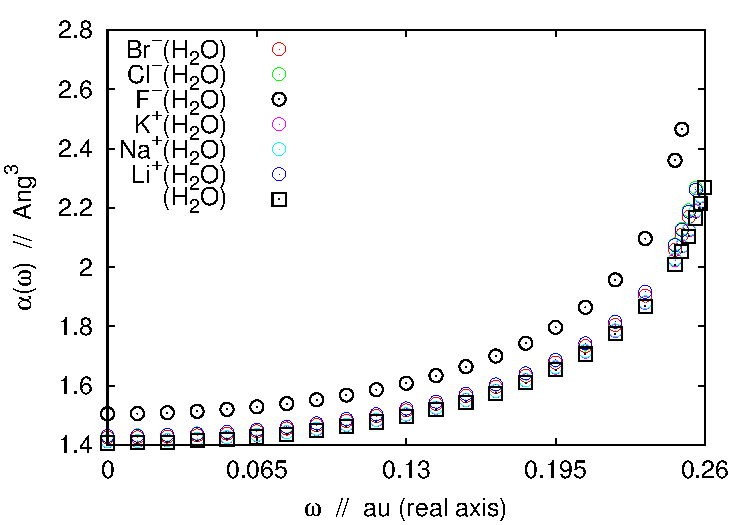
\includegraphics[width=0.98\linewidth]{images/all_polar_data.pdf}
 \end{center}
\caption[Dynamic polarizabilities of water in gas phase and ion-water dimer geometries]{Isotropic dynamic polarizabilities of water in native and ion-induced geometry for a 
range of 0 to 0.26 atomic units applied frequencies. Calculations were performed at the equations-of-motion coupled cluster to double excitations level with the aug-cc-pV5Z 
basis set using NWChem\cite{valiev2010nwchem}. Results are otherwise unpublished but are related to the calculations performed in Chapter \ref{ch3:sec0:level1}.}
\label{fig:dypol}
\end{figure}
    
   \subsection{\label{ch1:sec2:level3}Modern continuum solvation approaches}
    Recall that a solvation free energy model should consider ion/solvent interactions and solvent reorganization in the form of a cavity formation energy (sometimes referred 
    to as the solvophobic effect). Modern continuum solvent models are often built into \emph{ab initio} codes to add approximate solvation effects to molecules handled with 
    electronic structure theory. With the already high computational cost of many of these types of calculations, quality continuum solvation models are in extreme demand. 
    There are many of such methods out there, but the bulk of them are derived from the polarizable continuum model (PCM). This method expresses the solvation free energy in 
    the form,
    
    \begin{equation}\label{pcm}
        \mu^{ex} = \mu^{ex}_{elst} + \mu^{ex}_{disp-repulsive} + \mu^{ex}_{cavity}.
    \end{equation}

    A derivative method called the conductor-like polarizable continuum model (CPCM) and many other electronic structure solvation models involve small rearrangements of or 
    substitutions in the PCM equations. Despite the cavity and dispersion-repulsion terms showing up in Eq. \ref{pcm}, the PCM nor CPCM models handle dispersion or cavity 
    parts of the free energy very well\cite{pcmmodels}. Cavities in these theories are handled as a series of overlapping spheres centered at each of the atoms in the modeled 
    molecule(s). The PCM method is also really expensive with numerous derivatives to compute. CPCM simplifies the procedure greatly and performs very well with high dielectric 
    solvents. The CPCM model was used in a very recent single-ion free energy scale paper\cite{ishikawa2016quantum}.

    Truhlar et al. have developed a general solvation model which uses the full electron density of the molecule(s) to estimate solvent accessible surface area (SASA) and
    atomic surface tensions\cite{marenich2009universal}. These figures are related to the cavitation and dispersion-repulsion energies. Because the model actually attempts to 
    solve for cavitation and dispersion-repulsion interactions, it is often considered the best method for calculating solvation free energies -- the others essentially calculate
    the electrostatic part. The higher quality comes at the expense of computation time though. This model has been used to develop what was once was known as the `gold standard'
    scale in single-ion free energies, enthalpies, and entropies\cite{coe1998cpa1,kelly2006cpa}.

    Other models exist that are similar to those discussed above: COSMO, COSMO-RS, SMX (X=6, 8, 12, etc.), and DESMO\cite{lange2011simple}.
    
    Duignan and coworkers have developed a method recently which also solves for the terms given in Eq. 
    \ref{pcm} and applied it to the determination of single-ion solvation free energies, entropies, partial molar volumes, salt activities, osmotic coefficients, ion/ion potentials
    of mean force upon approach (investigating Collins' law of matching water affinities), and the free energy profile of the hydroxide and hydronium ions approaching the air/water 
    interface\cite{duignan2013continuum1,duignan2013continuum2,duignan2014collins,duignan2014ion,duignan2015hydronium,duignan2016ions}. Electrostatics are handled at the Born 
    level for simplicity but the authors also use the COSMO model (essentially any PCM model will work). Dispersion was handled through determination of the conventional C6, C8,
    and C10 coefficients from dynamic polarizability functions evaluated at the density functional level. They hope to treat dispersion using Green's functions in the future. A 
    simple cavity term is modeled as the product of a solvent-related constant and the excluded volume due to the ion. The volume term takes the distance to the first peak in
    the ion/water (oxygen-atom) radial distribution function from simulation or experiment as input. For ion-ion interactions, this volume excludes regions of overlap between the 
    ions. When the electrostatics are handled with COSMO, an approximate polarization energy is taken into account, else it is left out and suffers the usual difficulties associated 
    with Born solvation. For their study of hydroxide and hydronium approaching the air/water interface a surface potential of +0.13 V was assumed\cite{duignan2015hydronium}. I argue later
    why this assumption is very likely wrong and how their results change if using the potential I estimate in Chapter \ref{ch5:sec0:level1}. Other small errors may be due to the
    use of spherical cavities in the COSMO model for non-spherical ions. 
    
    Their results highlight the special importance of dispersion through $\mu^{ex}_{disp-repulsive}$ but also in the determination of $\mu^{ex}_{elst}$ from the COSMO model. 
    They show in Ref. \cite{duignan2014ion} that the 2\sur{nd} virial coefficient (inputs for both osmotic and activity coefficients -- this is a common extension of the Debye-H\"{u}ckel
    model to higher concentrations) for chaotrope-kosmotrope pairs are especially sensitive to the inclusion of electron correlation in the COSMO energy. The model overall 
    exhibits excellent qualitative agreement with experiment and shows the benefits of hybridizing approaches.
   
    I've reflected on a number of theoretical frameworks for modeling ion interactions with bulk solvent, interfaces, and other ions. These methods are of limited predictive
    value given their oversimplified description of solvation which lacks the granularity of explicit solvation models\cite{jungwirth2006airwat}. Even with extensive parameterization, 
    they struggle to mimic the strong and ion-specific local solvation forces. However, I mentioned (admittedly, in passing) that these models are appropriate for accounting for 
    long-range solvation effects which are almost entirely electrostatic in nature (at least in high dielectric solvents). Therefore, the pursuit is not necessarily in vain. Pairing these
    models with explicit handling of the first solvation shell(s) could lead to significant advances in the efficiency and accuracy of hybrid electronic structure/continuum
    approaches. This may also allow researchers to forego the use of periodic boundaries in simulation and simulate proper clusters free from artificial forces due to the
    boundary conditions. The quasichemical theory of solutions which I discuss in Chapter \ref{ch2:sec4:level4} and implement in Chapter \ref{ch6:sec0:level1} measures parts of 
    the free energy as the work to solvate a cavity of considerable size. Dipoles and quadrupoles forming at this junction can interact over a significant distance and may produce
    spurious and unaccounted errors when interacting with its image in a neighboring cell\cite{remsing2014lp}.
   
    Regardless, it is critical to stress that ion solvation is an inherently quantum mechanical problem due to the strong electric field around the ion and the importance of localized, 
    mutually polarizing, non-electrostatic forces, and other as yet undisclosed contributions.
    
  \section{\label{ch1:sec3:level1}Ion solvation is a quantum mechanical problem}
   This section motivates the use of electronic structure theory in the characterization of ion/ion and ion/solvent interactions. Though it is also instructive to point out that 
   ``well-parameterized classical models can capture important aspects of specific ion hydration, including high resolution single-ion thermodynamic quantities''\cite{pollard2016review}. 
   Indeed, the size of and timescales of simulations run today are virtually impossible to carry out at the electronic scale. So where does the need for very costly quantum chemistry
   come into play? Our successes in modeling ion solvation to spectroscopic and/or thermochemical accuracy can be used to train simpler models which can in turn be used to address
   matters requiring many atoms or long timescales.
   
   So what is going on in these inner shells that continuum models cannot reproduce (even in an \emph{average} sense)? In short, \emph{a lot}. There's a surprisingly large number
   of things to discuss on this matter so I'll break things down into a few categories (by no means an exhaustive list): 1) spectroscopic and theoretical evidences of chemical 
   character in the closest shells, 2) dynamical effects, particularly on solvent exchange between the inner shells, 3) nuclear quantum effects, 4) ions at interfaces, and 5) 
   some additional thoughts on atomistic modeling of non-electrostatic contributions for some perspective on how far we've come and the limitations of many existing force fields.
   
  \subsection{\label{ch1:sec3:level2}Chemical character of ion solvation}
   First, I re-establish the fact that monovalent ionic effects are limited to the first or second solvation shell. Markovich et al. measured the photoelectron spectra of 
   sequentially solvated ion/water clusters\cite{markovich1994photoelectron}. They measured the binding energy of the valence electrons of Cl\sur{-}, Br\sur{-}, and I\sur{-} ions
   with increasing cluster size, relating the change in the binding energy between subsequent cluster sizes to a stabilization energy. This figure was monitored with increasing
   cluster size to determine the size of the first solvation shell. The authors found this energy largely stabilized by a cluster size of \emph{n} = 6. Interestingly, each of the
   spectra reflected an increase of over 3 eV in the binding energy associated with solvation. A later study by Kurahashi et al. determined these values more accurately, with all
   of the respective binding energies increasing\cite{kurahashi2014photoelectron}. These authors observed that the change in the highest occupied molecular orbital (HOMO) binding 
   energy for the solvated water molecule decreases $\sim$1.3 eV relative to the gas phase water molecule. A redshift in other spectral features of water are observed as well and are
   linked in Ref. \cite{fransson2016x} to the formation of the hydrogen bonding network in bulk water. Intermediate these studies was one from Winter et al.\cite{winter2005electron}.
   The spectra in this paper are argued to have been superseded by those of Ref. \cite{kurahashi2014photoelectron}, but these authors also attempted to compute the binding energies
   using a combination of continuum and explicit particle methods. They found that continuum methods performed well for cations because solvent reorganization could be largely 
   neglected (the transition is from +1 to +2 charge), while for anions the continuum methods struggled (transition is from -1 to $\pm$0 charge). In water, the dipole orientation
   around a neutral cavity most resembles that of a cation\cite{wipff1999tatb,wipff2000tatb,wipff2001tatb,hummer1996}, leading to the poor comparison. A later study embedded partially
   solvated anion/water clusters in the same model and achieved significantly improved agreement with experiment\cite{dolgounitcheva2014microsolvation}. A separate study postulated
   that the neutral state of a particularly difficult case for band assignment in the spectrum of F\sur{-}/water more resembles F\sur{-}/H\sous{2}O\sur{+}\cite{canuto2010delocalized}, 
   likely owing to the large proton affinity of F\sur{-}\cite{kim2002bigall}. In a review by Seidel et al.\cite{seidel2016valence}, the vertical detachment energies (the binding 
   energies assuming no change in solute or solvent structure) are reported to correlate very well with the UV charge-transfer-to-solvent (CTTS) energy, even getting the Hofmeister 
   ordering of monovalent anions largely correct. Some of these authors recently reported on a new method for probing solvent-separated, solvent-shared, and contact ion pairs
   related to Collins' law of matching water affinities\cite{unger2016first}.
   
   It has been a longstanding goal across many fields to describe the dynamics of the solvated electron which is the simplest form of electron transfer reaction and so is a surrogate
   for understanding more complex chemistry. It is also believed to play a role in radiation induced damage of DNA\cite{coons2016hydrated}. Iodide is the most commonly used electron
   donor since it is relatively easy to excite and the simple nature of the neutral atom with no vibrational degrees of freedom reduces the number of variables to contend with in the 
   measurements\cite{kothe2015charge}. The solvated electron is generated by exciting the iodide valence orbitals to produce an I\sur{0}-e\sur{-} state (the nature of which is poorly
   understood)\cite{kothe2015charge}. The intermediate survives a reported 1-2 picoseconds before generating the solvated electron which relaxes after about 100-500 
   femtoseconds\cite{kothe2015charge}. Spectra of this sort have been produced both experimentally and theoretically for the halide series and even the sodium
   anion\cite{barthel2000direct,bradforth2002excited,galamba2009electronic,kim2000smallall,kim2002bigall,kloepfer1998femtosecond,lehr1999electron}. 
   
   But there's growing evidence that you don't need to excite the valence electrons of anions to see a portion of the excess charge spill out onto the 
   solvent\cite{angelina2013cov,attah2015structure,cordoba2011ctinhbonds,hynes2000cthalides,hynes2008ctnitrate,kim1999bigf,kim2000smallall,kim2002bigall,klein2005solutesolventct,lee2012ctice,mccoy2006prywaterf,mo2006polctqmmm,patel2010polarizability,rogers2010ctpolar,soniat2012ct,sarkar2013cthalideohraman,soniat2014ct_surf,rick2016polct}.
   Many of these studies relate intermolecular charge transfer (also known as charge displacement) to spectral shifts in IR or Raman stretching frequencies of the solvating water(s)\cite{xiong2010lowest}. 
   Another pair of studies (and the experimental and theoretical references therein) discuss modeling of the vibrational spectra for water when complexed with an 
   ion\cite{kamarchik2010quantum,puniyan2016theoretical}. This too is a very localized effect and can be so strong an influence that in the case of F\sur{-} and water, the ion is 
   often said to act as though it is ``prying apart'' the molecule\cite{collins2007review,mccoy2006prywaterf}. In a study by Choudhuri et al., the authors monitor the vibrational 
   frequency of the O-D stretch over the course of a simulation as the molecule diffuses away from F\sur{-}\cite{choudhuri2012first}. There is about a 200 cm\sur{-1} blueshift
   in the frequency as the molecule returns to the bulk. In a follow-up studies on Br\sur{-} and I\sur{-}, the authors noted that the O-D stretching mode actually decreased as the water
   diffused into the bulk\cite{karmakar2013first,karmakar2015water}. Diffusion coefficients in the first shell were also found to be greater than in the bulk, consistent with discussion
   above on the ``tumbling'' of waters around the alkali-halides measured with NMR\cite{karmakar2015water}. The use of heavy water minimizes the impact of nuclear quantum effects with 
   hydrogens.
   
   Using the quantum theory of atoms in molecules\cite{bader1990book}, I looked into this idea of F\sur{-} somehow ``prying apart'' the water molecule from the perspective of changes 
   in the electron density Laplacian (curvature) as a function of ion/water separation as in Ref. \cite{espinosa}. In Figure \ref{fig:laprho}, I show a previously unpublished plot
   of the curvature of the electron density measured at the junction between the halide anions and a bound water molecule. I monitor this quantity over a range of separations and compare 
   between two levels 
   of theory. In the atoms in molecules theory, a positive curvature indicates ionic character, while negative indicates covalent character. While not negative in value, it is very 
   interesting to note that the equilibrium geometry of the F\sur{-}/H\sous{2}O dimer falls on the part of the curve where the curvature becomes less positive with decreasing distance, 
   while both Cl\sur{-} and Br\sur{-} exhibit the opposite behavior. In Ref. \cite{espinosa}, this behavior is likened to a closed shell (electrostatic) interaction with emerging 
   covalent character. It's easy to rationalize that F\sur{-} forms stronger hydrogen bonds with water than the other halides. Kim et al. point out the high electronegativity and large 
   proton affinity of F\sur{-} relative to the other halides\cite{kim2000smallall}. But does the unique location of F\sur{-} on the Laplacian curve necessarily support this covalent
   narrative? It's possible, but we mustn't jump to conclusions. At the least I think it implies the exchange of density between the fragments is more fluid, but then again this behavior
   is difficult to characterize because there is no unique way to carve individual atoms out of a molecular system. Why is this definition of an ``atom'' better than another? That's a
   discussion beyond the scope of this thesis. Safe to say, Bader's theory does not impress some\cite{emptor} -- probably one of the most scathing reviews of anything I've ever seen.
   
   In spite of the difficulties associated with charge partitioning, partial charge transfer is believed to \emph{symmetrize} the first solvation shells by promoting internal ion 
   solvation over surface solvation\cite{rogers2010ctpolar,soniat2012ct}. Though induction is typically taken to include intramolecular polarization and intermolecular charge transfer, 
   high polarizability has been linked in several studies with increased solvation asymmetry (surface binding)\cite{carignano1997polarizable,dang1993molecular,herce2005surface,ohrn2007many,perera1992structure}. 
   Reconciliation may be found in an explanation that charge transfer reduces the excess charge on the ion, effectively making it harder and less polarizable. 
   
   Rick and coworkers have also argued that the cumulative charge transfer from the bulk to the interface leads
   to the apparent negative surface charge of air bubbles or oil droplets suspended in water\cite{vacha2011oil,soniat2014ct_surf,takahashi2005zeta}. However, the calculated excess 
   surface charge falls well short of those back-converted from experimental $\zeta$-potentials (about 60-150x smaller). The alternative hypothesis is OH\sur{-} adsorption at the 
   interface which is a \emph{highly} contentious topic I'll address later.
   
   The sheer number and diversity of structures reflected in many of the above studies and others such as Refs. \cite{ivanov2014stabilization,kemp2005theoretical,lambrecht2011exploring,lambrecht2012refined} 
   and those used in Chapter \ref{ch3:sec0:level1} very likely places an approximate description of local structure beyond the reach of continuum models as well.
   
\begin{figure}
 \begin{center}
  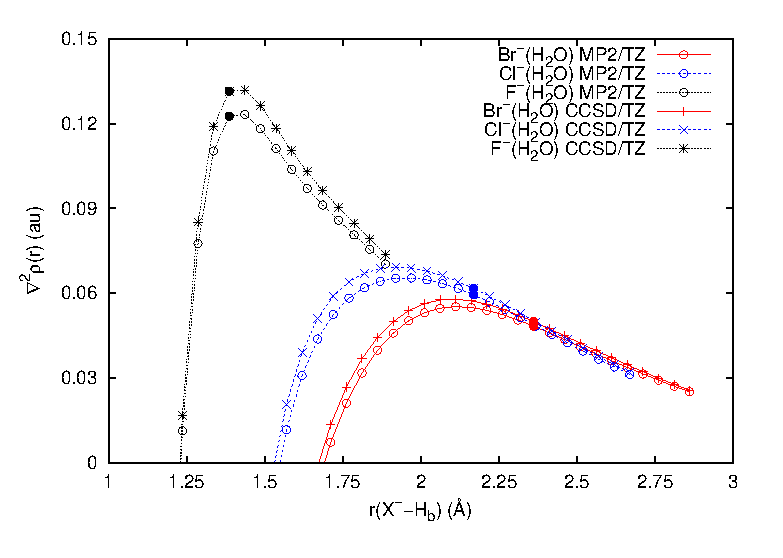
\includegraphics[width=0.98\linewidth]{images/laprho_v_distH.eps}
 \end{center}
\caption[Electron density curvature in halide/water dimers versus separation]{Laplacian (curvature) of the electron density in halide/water dimers measured at the bond critical point
linking the ion and water. A positive value indicates that density is not shared across the point, while a negative value denotes the opposite. According to Ref. \cite{espinosa}, the 
position of F\sur{-} on this curve is unique in that it coincides with the emergence of covalent character in the `bond.' Results are otherwise unpublished but are related to the 
calculations performed in Chapter \ref{ch3:sec0:level1}.}
\label{fig:laprho}
\end{figure}   
  
  \subsection{\label{ch1:sec3:level3}Temporal evolution of the solvation shell}
   Perhaps one of the most difficult aspects of ion solvation and possibly the best argument for molecular resolution is the \emph{softness} of the hydration shell conferred through
   the finite time of ion/solvent interactions, diffusion, and exchange between the first and second solvation shell. The earlier results of Heuft and Meijer suggest the first hydration 
   shell is rather \emph{hard} around F\sur{-} and Cl\sur{-} -- in this sense meaning sharply cut off from the rest of the solution\cite{heuft2003cl,heuft2005f}. Though they find the
   solvation shell around I\sur{-} to be rather unstructured with rapid exchange between shells\cite{heuft2005i}. Karmakar et al. in their series of studies on halide ion solvation 
   also addressed the diffusion coefficients of ion-bound waters, the lifetime of hydrogen-bonds, and dynamics of water reorientation in the first 
   shell\cite{choudhuri2012first,karmakar2015water}. The dynamics of first shell waters was found to fall into three distinct timescales: short-time relaxation dynamics ($\sim$100 fs), 
   lifetime of the X\sur{\pm}$\cdot\cdot\cdot$H bond (F\sur{-} ($\sim$7.5 ps) > Cl\sur{-} ($\sim$3 ps) $\approx$ Br\sur{-} ($\sim$3-4 ps) > I\sur{-} ($\sim$2-3 ps) > H\sous{2}O 
   ($\sim$1-2 ps)\cite{bankura2014structure,ojha2015ultrafast}). The somewhat labile nature of the coordination shell is supported also by the work of Laage and 
   Hynes\cite{laage2007reorientional}. A somewhat dated study by Kozi{\'n}ski et al. estimated the lifetime of the hydrogen bond between water and CN\sur{-} to be about 2.9 
   ps\cite{kozinski2007vibrational}. Interestingly these changes come with no discernible change in the dipole moments of the waters between the first and second 
   shell\cite{heuft2003cl,heuft2005f,heuft2005i,krekeler2006density}.

   Water residence times also differ significantly across the halide series (F\sur{-} ($\sim$26 ps) > Cl\sur{-} ($\sim$20 ps) $\approx$ Br\sur{-} ($\sim$20 ps) > I\sur{-} ($\sim$14-16 ps)). 
   As shown by Heuft et al., the solvation shell of the ion when undergoing solvent exchange will take on unique characteristics not observed for low energy conformers used to parameterize 
   continuum and simple all-atom models\cite{heuft2003cl,heuft2005f,heuft2005i}. F\sur{-}, for example, will take on a short lived hexahydrate coordination sphere before returning one of
   the waters to the bulk\cite{heuft2005f}. The inherent flexibility in the coordination number can only be reasonably approximated with an all-atom model and then again only 
   \emph{accurately} with electronic structure resolution. Residence times are also critically important in understanding the dynamics of solvation around proteins\cite{pal2002biological}
   which can be modified by the presence of electrolytes (and hence the Hofmeister series).
   
   These results also stress the importance of including dispersion effects in density functional modeling of hydrogen bonding dynamics in electrolyte 
   solutions\cite{bankura2013hydration,bankura2015systematic}. However, some care must be taken to be sure the corrected functional doesn't over/under structure water, as is common.
   Recent simulations also highlight the critical importance of dispersion in modeling the first shell of Na\sur{+} and K\sur{+} to accurately determine coordination numbers from the 
   integral of the radial distribution function\cite{bankura2014hydration}. A systematic review of the challenges ion solvation pose for density functional theory can be found in 
   Ref. \cite{soniat2015dispersion}.
   
  \subsection{\label{ch1:sec3:level4}Nuclear quantum effects}
   Much of the simulation work discussed above was done with heavy water, but why? As the proverb goes, ``when it rains it pours.'' Extending beyond the usual difficulties in 
   describing the electronic wave function, the small mass of the proton means nuclear quantum effects play an important role in hydrogen bonded systems.
   Nuclear quantum effects (NQEs) are purported to increase the mobility of both H\sur{+}\cite{marx2000solvated} and OH\sur{-}\cite{tuckerman2002nature}, which may be important in
   proton shuttling along membranes and hydrophobic surfaces\cite{zhang2012water}. NQEs are also likely responsible for a number of anomalous behaviors in liquid water and in 
   ice\cite{pamuk2012anomalous}. 
   
   Nuclear effects are generally thought to occur in hydrogen bonds through two competing modes 1) proton sharing through a stretching mode
   (HO$\cdot\cdot\cdot$H$\cdot\cdot\cdot$O$\cdot\cdot\cdot$H\sous{2}) and 2) distortions in the bond due to rotation of the participating molecules\cite{ceriotti2016nuclear}.
   As a general rule of thumb, nuclear effects weaken weak hydrogen bonding interactions and strengthen stronger ones\cite{ceriotti2016nuclear,guo2016nuclear}. You might think this 
   makes NQEs more important for anion solvation -- but it has actually been found to be more important for Li\sur{+} than F\sur{-} due to the competing effects discussed 
   above\cite{wilkins2015nuclear}. Suzuki et al. have also found that NQEs in small F\sur{-}/water clusters led to elongation of the hydrogen bond distance\cite{kawashima2013ab}. 
   Wang et al. observed similar behavior in small Cl\sur{-}/water clusters.
   
   These effects can be included for both quantum and classical descriptions of electrons. Including NQEs generally improves the quality of simulations across a broad range of 
   temperatures\cite{vega2010heat}. In conventional \emph{ab initio} dynamics a 30--50 K increase in the temperature has been found to mimic NQEs and corrects the radial 
   distribution function (rdf) of liquid water at 300 K (simulation temperature is 330--350 K) and slightly decreases the overall structuring (lower peak in 
   rdf)\cite{morrone2008nuclear}. However, this is a questionable approximation\cite{weber2010communication}. Additional influences of NQEs are addressed in a recent
   review\cite{ceriotti2016nuclear}.

  \subsection{\label{ch1:sec3:level5}Ion adsorption at the air/water interface}
   Ion adsorption at the air/water interface is a relatively recent discovery. For quite some time it was believed that all ions were repelled from the interface because 1)
   the surface tension of water increases with the addition of most inorganic salts predicting a negative surface excess by the Gibbs adsorption isotherm and 2) the primitive
   dielectric models predict that ions solvated in a higher dielectric medium are repelled from the interface due to an image charge force. The air/water interface was believed 
   to be ion-free and relatively inert\cite{ishiyama2014theoretical,jungwirth2006airwat}. This all changed with Hu et al.\cite{hu1995reactive} who noticed that the kinetics of Cl\sous{2} and 
   Br\sous{2} uptake in solutions of NaI and NaBr did not fit the rate predicted by a bulk-phase reaction mechanism (X\sous{2} + Y\sur{-} $\rightarrow$ XY + X\sur{-}). The 
   authors inferred significant surfactant behavior of Br\sur{-} and I\sur{-} as Y\sur{-} to fit their model to their experimental measurements. Since then, research into the 
   surface activities of inorganic ions and the acid/base chemistry of the water surface has become wildly popular.
   
   Cheng et al., Netz et al., and Ou et al. have found strong correlation between anion affinity for the air/water interface and ion radius\cite{cheng2006experimental,netz2009ionsinterfaces,ou2016molecular}. 
   Researchers more commonly ascribe surface propensity to 
   polarizability\cite{jungwirth2002airwat,jungwirth2006airwat,pegram2006partitioning,pegram2007hofmeister,petersen2005adsorption,petersen2006nature,wick2007effect}.
   Polarizability (or an especially large dipole on the waters in nonpolarizable models) was found to be a critical factor in determining whether this behavior would be seen
   from molecular dynamics trajectories\cite{stuart1996effects}. However, the role of polarization in polarizable force fields such as AMOEBA may be overestimated somewhat, 
   exaggerating the role polarization may play here\cite{rogers2010ctpolar}. There may be several competing effects also including surface capillary waves, desolvation, cavity 
   formation, and the surface potential across the air/water boundary\cite{ayse2012,ben2016interfaces,rane2016understanding}. 
   
   Surface affinity appears to also change with the counterion in solution\cite{cheng2012ambient,hua2014cation,tissot2015cation}. The ordering of ions in the double layer can
   switch when the anion is strongly kosmotropic and the depth of the region of ion accumulation/depletion at the interface can extend to more than a nanometer into the solution\cite{brown2015ion}. 
   However, the region of enhanced ion density relative to the bulk is more commonly limited to about half that distance. This is based on density profiles of the ionic species 
   extracted from molecular dynamics simulations and also the anion/cation ratios probed at various depths by high-pressure photoelectron spectroscopy\cite{jungwirth2006airwat}. 
   The density profiles and spectra also show that the net charge density profile over the interfacial region produces a negative surface excess. The depleted layer a few water 
   diameters deep more than makes up for the surface active layer(s) above it, an illustration of this is given in Ref. \cite{jungwirth2006airwat}. 
   
   Hua et al. have also shown that the interface can be depolarized at sufficiently high concentrations of surface active ions; the authors used 1.7 M perchlorate in this case\cite{hua2013surface}. 
   Depolarizing the interface with an applied voltage while monitoring relative surface excesses may be used to approximate the contact/surface potential essential to the
   establishment of an absolute single-ion thermodynamic scale\cite{conboy1997shg_tatb}.

   While the surface activity of some ions is well-established, there are still some lingering issues with quantifying the enhancement (see Refs. 253--256 in Ref. \cite{bjorneholm2016water})
   due to discrepancies between X-ray methods, sum-frequency (SFG) and second harmonic generation (SHG) spectroscopies, and theoretical approaches. Adsorption of hydronium 
   or hydroxide ions at the interface remains an extremely contentious topic of research, however. Hydroxide adsorption at the interface is suspected because 1) the 
   $\zeta$-potential in neat water is negative as mentioned previously, 2) the surface tension of a freshly formed air/water interface relaxes from 80--100 mN/m to 73 mN/m 
   in about 1 ms (about the same time required for OH\sur{-} buildup due to autolysis and diffusion); competing mechanisms occur on ps (too fast) and s (too slow) timescales\cite{liu2012surface},
   3) other anionic and/or fatty acid impurities are not observed at the air/water interface in SFG/SHG experiments\cite{jena2012surface}, 4) the isoelectric point of the air/water
   interface is at pH 2.5--4\cite{beattie2014surfacid,buch2007surfacid,liu2012surface,mishra2012surfacid}, and 5) the surface tension of water is largely pH-independent from 
   pH 4--13. This last point does not necessarily point to one ion over the other making an appearance at the interface (as noted in Ref. \cite{jungwirth2015comment}), but 
   demonstrates the robust nature of the surface charge, strengthening the conclusions generated from other studies. 
   
   Theoretical studies and SFG/SHG experiments typically predict hydronium adsorption at the interface\cite{buch2007surfacid,mucha2005unified,petersen2008liquid,tse2015propensity,willow2011nh4+}.
   A notable exception is a study by Mundy et al. which found a small $\sim$0.6 kcal/mol attraction of OH\sur{-} to the air/water interface\cite{mundy2009hydroxide}. The 
   free energy profile of H\sous{3}O\sur{+} is more often shown to have a minimum near the interface, while the OH\sur{-} profile is purely repulsive. This is interpreted to
   reflect the loss of water contacts by OH\sur{-} and a favorable enthalpic contribution through exclusion of H\sous{3}O\sur{+} from the bulk\cite{tse2015propensity}. However, 
   a study by Brorsen et al. made the interesting observation that hydronium did not prefer surface solvation when the ion and water were modeled at the \emph{ab initio} level, 
   but did when the water was handled with the TIP5P water model\cite{brorsen2014surface}. This is a 5-point classical point charge model which is known to have almost no 
   surface potential contribution\cite{remsing2014lp}. The surface potential is believed to play a role in ion adsorption at interfaces\cite{ayse2012,duignan2015hydronium}.
   The surface potential I derive in Chapter \ref{ch5:sec0:level1} acts at about $\frac{1}{2}$ its full value near the interface and if included in the study of Tse et al. in Ref. 
   \cite{tse2015propensity} reverses their prediction. Adsorption of the OH\sur{-} ion is selected over H\sous{3}O\sur{+} by $\sim$4--6 kcal/mol, similar to that discussed 
   in the conclusions of Ref. \cite{liu2012surface}. This difference corresponds to a $\sim$10\sur{4} preference for OH\sur{-}. This is consistent with the pH needed to 
   neutralize the surface of water.
   
   There are also several complicating factors with surface sensitive spectroscopies which are in need of resolution: 1) the signal can be convoluted by poorly understood 
   quadrupolar or bulk solvent contributions\cite{carrier2016ionsatowinterface,kundu2016bend}, 2) the probe depth is poorly characterized and appears to be able to change with
   ionic strength from about 1 nm to over 1 $\mu$m\cite{gonella2016second}, 3) the signal which is thought to measure surface adsorption does not necessarily translate back to
   propensity\cite{carrier2016ionsatowinterface}, and 4) the OH\sur{-} may (weakly) or may not be visible to SFG/SHG\cite{imamura2014molecular,mishra2012surfacid}. These are
   important concerns to address considering that SFG/SHG are also used to probe structure of the air/water, oil/water, and other non-aqueous solvent
   interfaces (e.g., directionality of the O-H bond: pointing into vapor phase or into bulk?)\cite{conboy1997shg_tatb,luo2015electrobreak,wang2016surface}. Issues with 
   theoretical approaches are typically related to the small size of simulations and the poor performance of classical force fields for this type of work\cite{beattie2014surfacid}.
   
   See Refs. \cite{bjorneholm2016water,bonn2015molecular,ishiyama2014theoretical,wang2016surface} for additional reviews on interfacial effects and surface sensitive 
   spectroscopies and Ref. \cite{agmon2016protons} for a recent survey of literature related to the ongoing debate about H\sous{3}O\sur{+}/OH\sur{-} surface affinity.
   
  \subsection{\label{ch1:sec3:level6}Additional comments on modeling non-electrostatic forces}
   Polarizable force fields are hit and miss with over-polarization being a pretty severe problem in classical models\cite{vdS2011surfacepref} in comparison with more realistic 
   quantum models\cite{baer2011toward}. Another concern is whether the model should make use of full gas phase or reduced condensed phase ion polarizabilities\cite{masia2009polarize,patel2010polarizability}.
   The popular AMOEBA force field has seen some refinement in the parameters over the years to combat these 
   issues\cite{laury2015revised,ren2003amoeba,ren2003amoebaion,amoeba,ponder2010znamoeba,wang2013systematic} but still over-polarizes anions. This can be corrected by variation 
   of a damping parameter employed in the self-consistent polarization calculation\cite{pollard2014cpa1}. However the adjustment necessarily distorts the solvation structure and 
   thermodynamic quantities without full re-parameterization. In the calculations I perform in Chapter \ref{ch5:sec0:level1}, the F\sur{-}/water peak in the radial distribution
   function is pushed about 0.25 \AA~beyond that when using the default model parameters. This was a fortuitous change for us however as I discuss in that chapter.
   
   Additionally, the AMOEBA assigned polarizability of the particles is static when I have shown previously that it can in fact change. The effect may not be as pronounced in 
   water where the dipoles of waters in the first shell may not differ drastically from those more distant from the ion, but this is not the case in every solvent\cite{ayse2016ecpc}, 
   also see Chapter \ref{ch4:sec0:level1}. The model of Steve Rick and coworkers reviewed in Ref. \cite{rick2016polct} I think represents the state of the art in force field 
   modeling. It incorporates two major improvements over AMOEBA in particular. 1) Polarization is handled using a Drude oscillator which adjusts the polarizability dynamically
   based on the environment and takes gas phase polarizabilities as input and 2) the model incorporates a simple and efficient description of charge transfer. Stuart and Berne 
   used a similar model, concluding that the larger dipole moment of these water models as compared to nonpolarizable ones made for a more accurate representation of both the
   dielectric and dynamic properties of liquid water\cite{stuart1996effects}. Fortunately, despite the deficiencies in polarizable force field models, they are often 
   qualitatively correct and have proven exceedingly useful in addressing selective adsorption of ions at the air/water interface.

   The van der Waals (vdW) potential in classical force fields, meanwhile, is a kind of mathematical Frankenstein composed of dispersion, exchange repulsion, surface potential
   effects, and corrections for all manner of uncategorized errors necessary to produce a better fit to a desired property. Fits of interaction parameters may be done against a
   dizzying array of experimental variables\cite{nezbeda2016recent} and sometimes the parameters of cations and anions are fit to different experimental quantities, best 
   exemplified in Ref. \cite{netz2009}. Nezbeda et al. have published a recent review on the difficulties of force field development especially as it pertains to the theoretical
   prediction of electrolyte solubility\cite{nezbeda2016recent}. The authors (and I) believe some standardization is desperately needed. My work in Chapters \ref{ch5:sec0:level1} 
   and \ref{ch6:sec0:level1} defines and characterizes a separate surface potential effect which also can serve to clean up the vdW potential in \emph{all} force fields a bit. 
   These papers also provide a road map for relating simulated quantities to experiment. Surface potential effects and single-ion thermodynamics are addressed in the next section.

  \section{\label{ch1:sec4:level1}Surface potential effects on the solvation of ions}
   Earlier I argued that the determination of an accurate single-ion thermodynamic scale was essential in our pursuit to finally begin to unravel the specific ion effects. What
   follows is a summary of the state of affairs in establishing such scales in aqueous and two energy storage related media, namely ethylene and propylene carbonate.

  \subsection{\label{ch1:sec4:level2}The single-ion scale}
   Solvation properties of neutral particles can be uniquely determined through experimental methods as long as an accurate equilibrium constant between gas and solution phase
   partitioning can be established. This applies also to ion \emph{pairs} wherein one ion neutralizes the net charge of the other. Solubility measurements can also be used to 
   establish solvation properties though the lattice energy of the salt must be removed to convert solution properties to solvation ones\cite{peruzzi2015solvation}, 
   see the representative thermodynamic cycle in Figure \ref{fig:thermocycle}. A list of lattice energies is found in Ref. \cite{marcus2012ions} on page 33. 

% trim .... left, bottom, right, top
\begin{figure}
 \begin{center}
  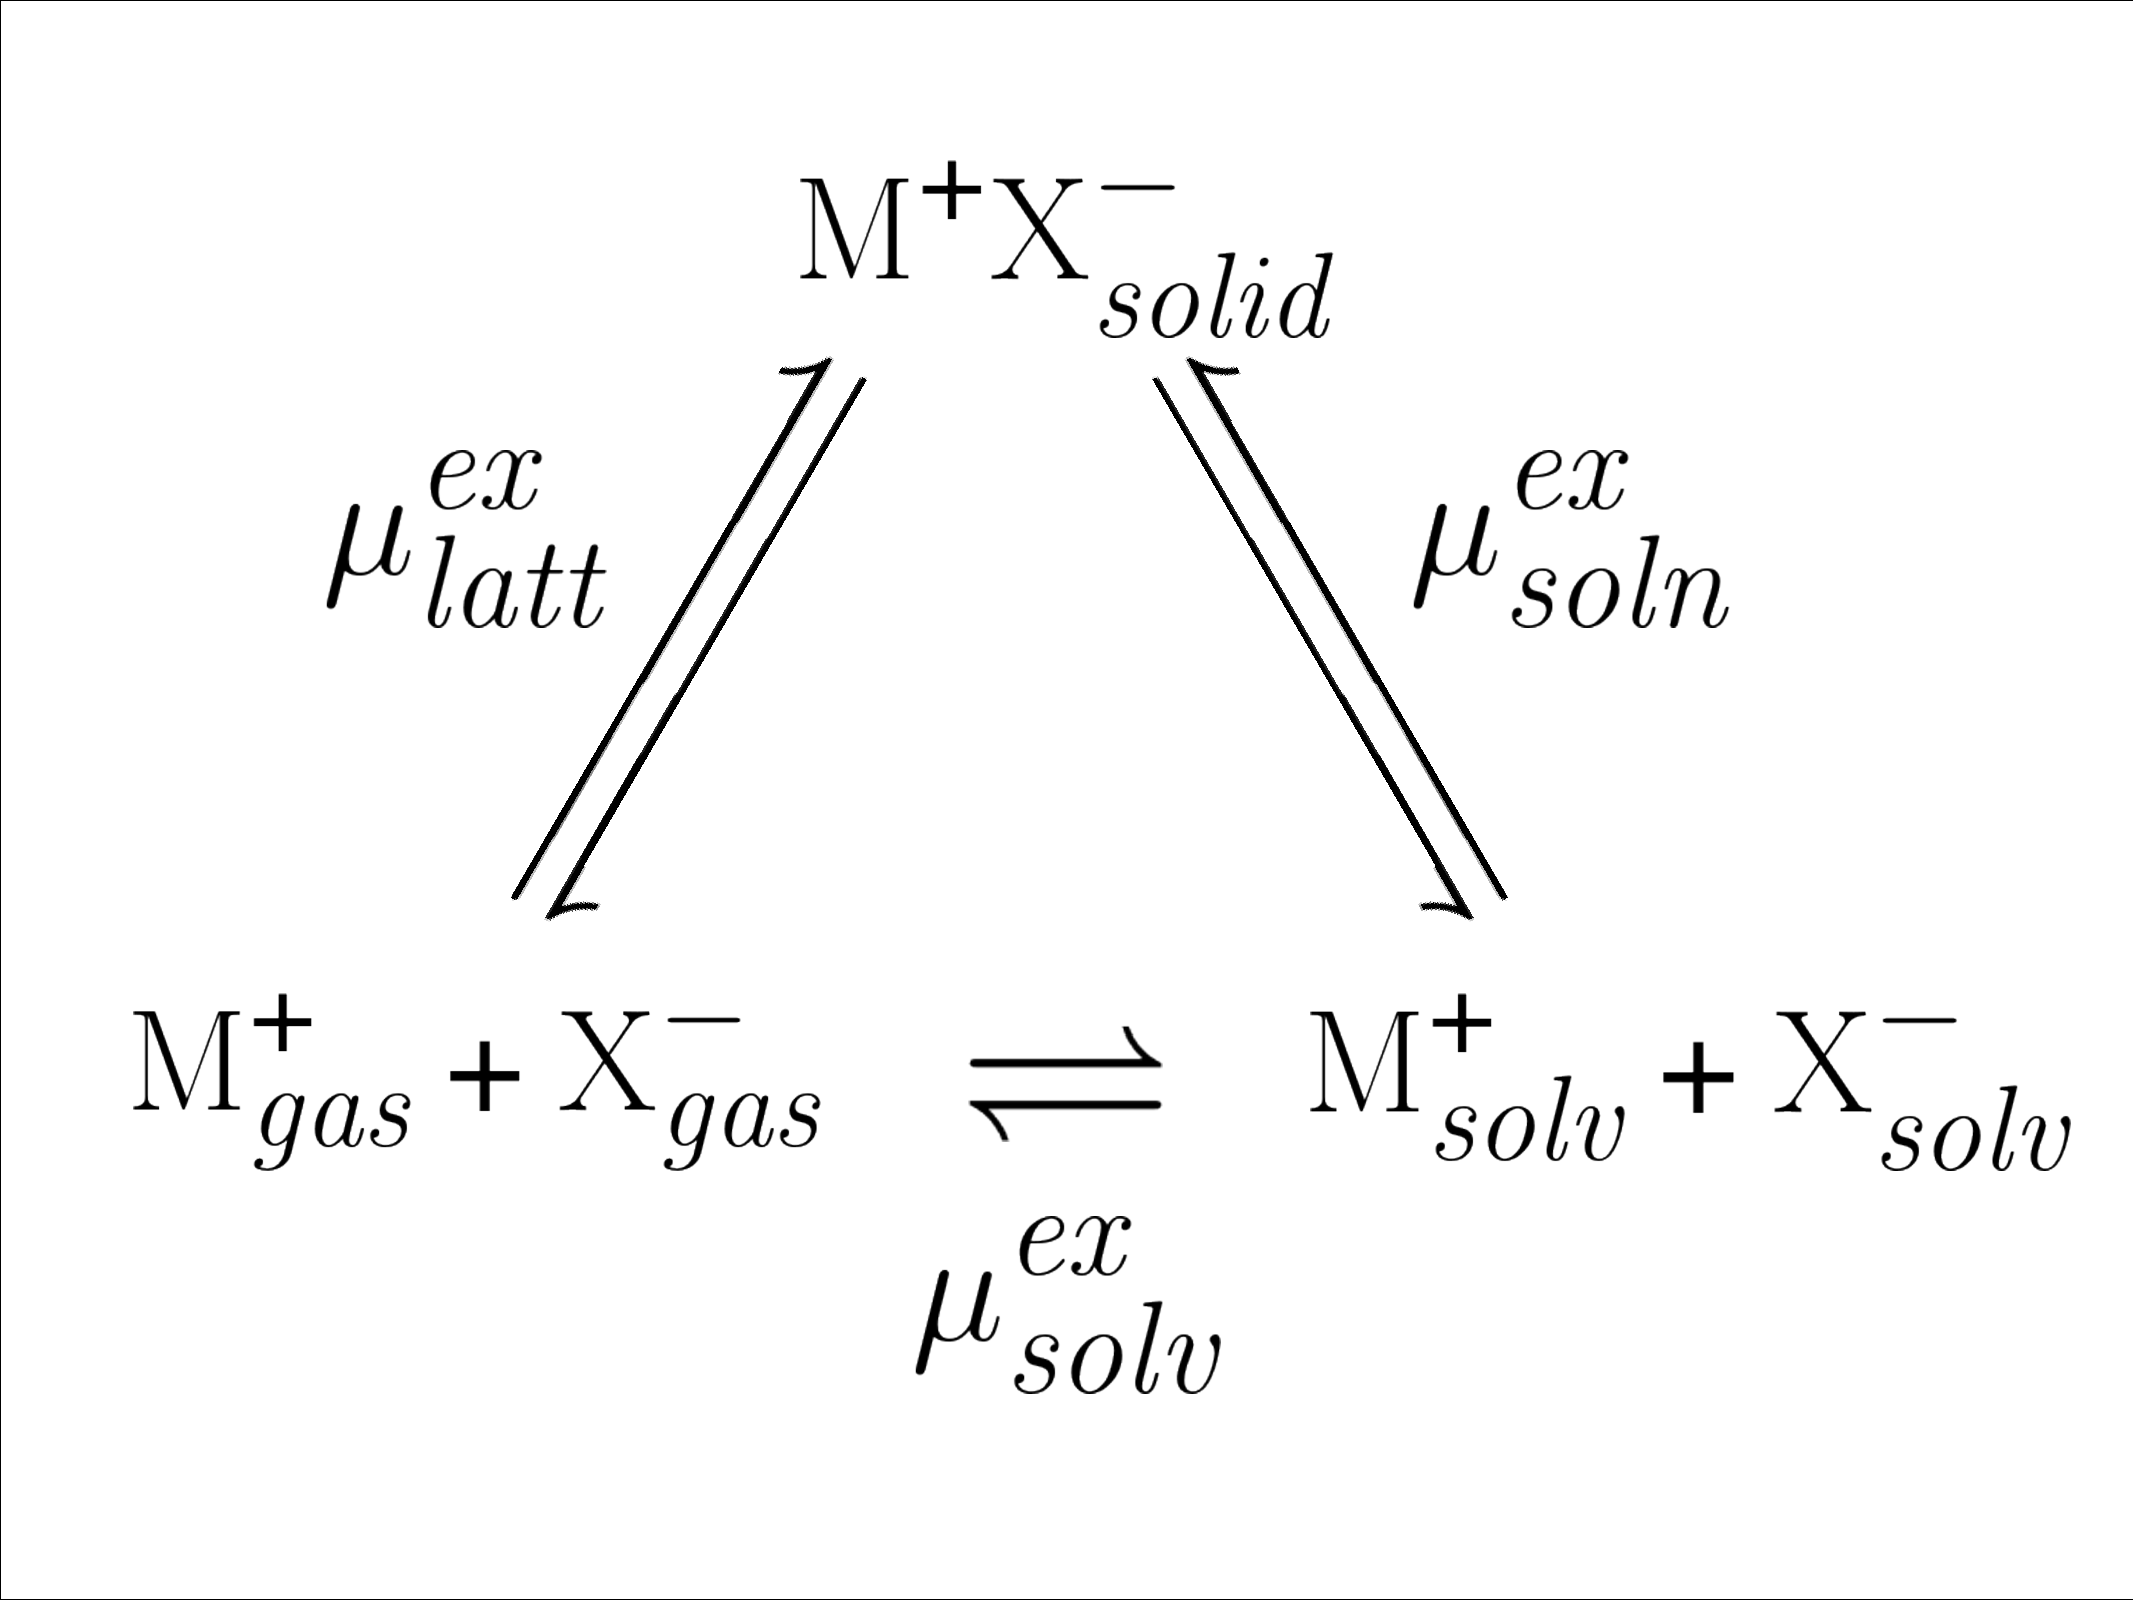
\includegraphics[width=0.98\linewidth,trim=0.2cm 2.2cm 0.2cm 0.2cm,clip=true]{images/thermocycle.pdf}
  \caption[Schematic of the thermodynamic cycle]{A thermodynamic cycle relates the lattice free energy, solution free energy, and solvation free energy through a series of 
  transitions/transfers.}
  \label{fig:thermocycle}
 \end{center} 
\end{figure}     
   
   The solvation free energy and related properties are a specific case of transfer free energy from vapor into solution rather than between two solutions. More generally, 
   transfer experiments can be conducted in mutually saturated solvents that are in contact with one another or in the pure solvent. The choice can often lead to very different 
   results as the more hydrophilic ions tend to coextract with residual waters into the non-aqueous phase\cite{rose2009, darvas2011, darvas2013}. Electrochemical
   methods can be used as well\cite{gomer1977experimental,randles1956real}. More recently advanced mass spectrometry setups have been used to determine sequential hydration
   enthalpies and based on my results from Chapter \ref{ch5:sec0:level1} may be able to establish the most accurate thermodynamic scale to date\cite{wheeler2015hydration,bard2014electroanalytical}.
   A list of pair free energies for alkali/halide salts is shown in Table 6 of Ref. \cite{lamoureux2006absolute}. There is typically very little variation in the pair
   solvation properties between different measurements and these are known to high accuracy\cite{ren2003amoebaion}. 
   
   The solvation free energy for a salt is very simple,
   
   \begin{equation}\label{eq:pairmu}
       \mu^{ex}_{pair} = \mu^{ex}_{P,b} + \mu^{ex}_{N,b},
   \end{equation}

   \noindent so long as we don't try to separate the contribution made by each ion individually. Once we try to do that, the best we can come up with is the \emph{conventional}
   scale where everything is measured relative to the proton,
   
   \begin{equation}
     \mu_N^{ex,con} =  \mu^{ex}_{N} + \mu^{ex}_{\mathrm{H}^+} = \mu^{ex}_{N,b} + \mu^{ex}_{\mathrm{H}^+,b}
     \label{eq:conv1}
   \end{equation}

   \noindent for a negatively charged ion and

   \begin{equation}
     \mu_P^{ex,con} =  \mu^{ex}_{P} - \mu^{ex}_{\mathrm{H}^+} = \mu^{ex}_{P,b} - \mu^{ex}_{\mathrm{H}^+,b}
     \label{eq:conv2}
   \end{equation}   
   
   \noindent for a positive one. This is because with the exception of mass spectrometry, no other experimental method is able to make measurements on isolated charges. Even
   then, these studies are limited to the determination of sequential hydration enthalpies for clusters extending just beyond the first shell. It's more common to split
   bulk thermodynamic and electrochemical measurements using an extrathermodynamic assumption to solve for the proton quantities and thus all others through Eqns. \ref{eq:conv1}
   and \ref{eq:conv2}. Some of the more cited of these are reviewed below.
  
   Another problem in the determination of a single-ion scale is the fact that dragging charges across solution interfaces also incurs a contribution from the electrostatic 
   potential associated with the interface. This is often called the surface potential, phase potential, or contact potential\cite{lamoureux2006absolute,pratt1992contact}. 
   Pioneering minds like Gibbs and Guggenheim long ago ruled this pursuit out concluding potential shifts experienced by single ions moving across interfaces are not 
   thermodynamically measurable\cite{gibbs1,guggenheim28,guggenheim-td}.
   
   Nevertheless, the real electrochemical solvation free energy for a single ion is expressed as\cite{aquaincognita2014,pratt1992contact,fawcett,beck2013sp},
   
  \begin{equation} 
    \mu_X^{ex} = \mu_{X,b}^{ex} + q\phi_{np}
    \label{eq:echemmu1}
  \end{equation}

  \noindent where $\mu_{X,b}^{ex}$ is the bulk hydration free energy (that includes all interactions of the ion with water except for the surface potential 
  contribution). $\mu_{X,b}^{ex}$ is also called the \emph{intrinsic} free energy\cite{hunenberger2011sp} and $\mu_X^{ex}$ the \emph{real} free energy. Similar
  nomenclature is extended to the hydration enthalpy which is
  
  \begin{equation}
    h_X^{ex} = h_{X,b}^{ex} + q\phi_{np} - qT\left(\frac{\partial \phi_{np}}{\partial T}\right)_P
    \label{eq:echemh1}
  \end{equation}

  \noindent and the hydration entropy\cite{lynden1997hydrophobic} is

  \begin{equation}
    s_X^{ex} = s_{X,b}^{ex} - q\left(\frac{\partial \phi_{np}}{\partial T}\right)_P.
    \label{eq:echem1}
  \end{equation}

   \noindent The enthalpy and entropy add a new term which corresponds to the temperature derivative of the surface potential. The enthalpy also contains a contribution
   made by the surface potential itself, while the entropy does not. The surface potential contributions cancel out in Eqns. \ref{eq:pairmu}--\ref{eq:conv2} leading to the
   excellent agreement among the various methods for pair and conventional free energies and the like. These figures become less agreeable when the pair quantities are 
   divided into their respective single-ion scales, see Figure 2 in Ref. \cite{lamoureux2006absolute}. With this in mind, let's review some of the more commonly cited 
   extrathermodynamic assumptions.
   
   \begin{itemize}
       \item Marcus scale\cite{marcus1985book} using the method of Halliwell and Nyburg\cite{halliwell1963enthalpy} for the proton enthalpy and Conway's bulk proton solvation
       entropy\cite{conway1978evaluation}. The values are -254.3 kcal/mol, -261.5 kcal/mol, and -24.0 cal/mol-K for the free energy, enthalpy, and entropy respectively.
       \item Born model with adjusted radii (Latimer-Pitzer-Slansky)\cite{ashbaugh2008lps,latimer1939freenergy}, giving identical results to the Marcus method.
       \item Assuming equal solvation entropies between H\sur{+} and OH\sur{-} (s\sursous{ex}{H\sur{+}} = s\sursous{ex}{OH\sur{-}})\cite{schmid2000blkfe}. The proton 
        quantities are -251.4 kcal/mol, -257.6 kcal/mol, and -20.7 cal/mol-K for the free energy, enthalpy, and entropy respectively.
       \item Assuming very large, ligand-screened, hydrophobic ions of opposite charge  have the same solvation properties in \emph{every} solvent 
       (tetraphenylarsonium/tetraphenylborate, TA\sur{+}/TB\sur{-})\cite{marcus1987tatb}. These results are slightly shifted from those of Marcus above. The hydration enthalpy
       of the proton is -263.6 $\pm$ 1.7 kcal/mol. The Conway entropy is assumed again\cite{conway1978evaluation}. The hydration free energy is then -256.4 kcal/mol.
       \item The extrapolation of gas phase, sequential hydration properties to the bulk via the cluster pair approximation\cite{coe1998cpa1,coe2001cpa2,coe2002cpa3,kelly2006cpa}. 
       The values here are very different from those above: -265.9 kcal/mol, -274.9 kcal/mol, and -30.0 cal/mol-K for the free energy, enthalpy, and entropy respectively.
       More recent re-evaluations with the method have led to a new set of recommended values: -265.3 kcal/mol, -275.3 kcal/mol, and -33.3 cal/mol-K\cite{donald2010expand_cpa}.
   \end{itemize}
   
   The last result here very clearly differs from the others, but it is most certainly not the only one in that range, more are listed in Ref. \cite{ishikawa2016quantum}. This 
   difference extends to the other ions when these proton values are inputted into the \emph{conventional} free energy scale above (again, see Figure 2 in Ref. \cite{lamoureux2006absolute}). 
   Previous efforts have determined that all but the last of the listed approaches above \textbf{excludes} the charge-dependent, linear surface potential term in the free 
   energy\cite{asthagiri2003absolute,ashbaugh2008lps,beck2013sp,shi2013length}. I refer to these values as the ``bulk'' quantities from Eqns. \ref{eq:echemmu1} -- \ref{eq:echem1}. 
   Could the surface potential in Eqns. \ref{eq:echemmu1} and \ref{eq:echemh1} be the piece that links these scales together and explains why they appear shifted from one another? 
   What even is this surface potential contribution? These questions are central to my work in Chapter \ref{ch5:sec0:level1}.

  \subsection{\label{ch1:sec4:level3}The air/water surface potential}
   In reference to Figure \ref{fig:potqct}, $\phi\sous{sp}$ is the total surface potential across the air/water interface and $\phi\sous{lp}$ is the imaginary inner interface 
   across the solvent/solute boundary where the electrostatic potential differs from that of the bulk solvent. I'll refer to $\phi\sous{lp}$ as the local potential, a
   recent study has also identified this potential\cite{remsing2016role}. $\phi\sous{sp}$ has been characterized by simple point charge models, electrochemical experiments, 
   density functional calculations, and complex electron holography measurements with values ranging from -1 to nearly +4 V\cite{leung2009sp_mag}. The origin of this tremendous 
   spread was beautifully illustrated by Kathmann et al.\cite{kathmann2011sp}. To summarize, density functional calculations and high energy electron holographic measurements
   have access to interrogate the full electron density while electrochemical measurements samples from the intermolecular density which leads to a smaller observed potential 
   jump relative to the vacuum. Contributions to this potential were found to be almost entirely due to molecular quadrupoles. A large cancellation of $\phi\sous{sp}$ occurs 
   crossing the solvent/cavity interface as $\phi\sous{lp}$ is of similar magnitude but opposite sign. Their sum produces the net potential ($\phi\sous{np}$), which is reduced
   from $\phi\sous{sp}$ and $\phi\sous{lp}$ by about an order of magnitude\cite{harder2008origin,kathmann2011sp,beck2013sp,remsing2014lp}. The shift in free energies due to interfacial 
   potentials has also been observed in several studies\cite{lamoureux2006absolute,ashbaugh2008lps,beck2013sp}.
   
\begin{figure}
 \begin{center}
  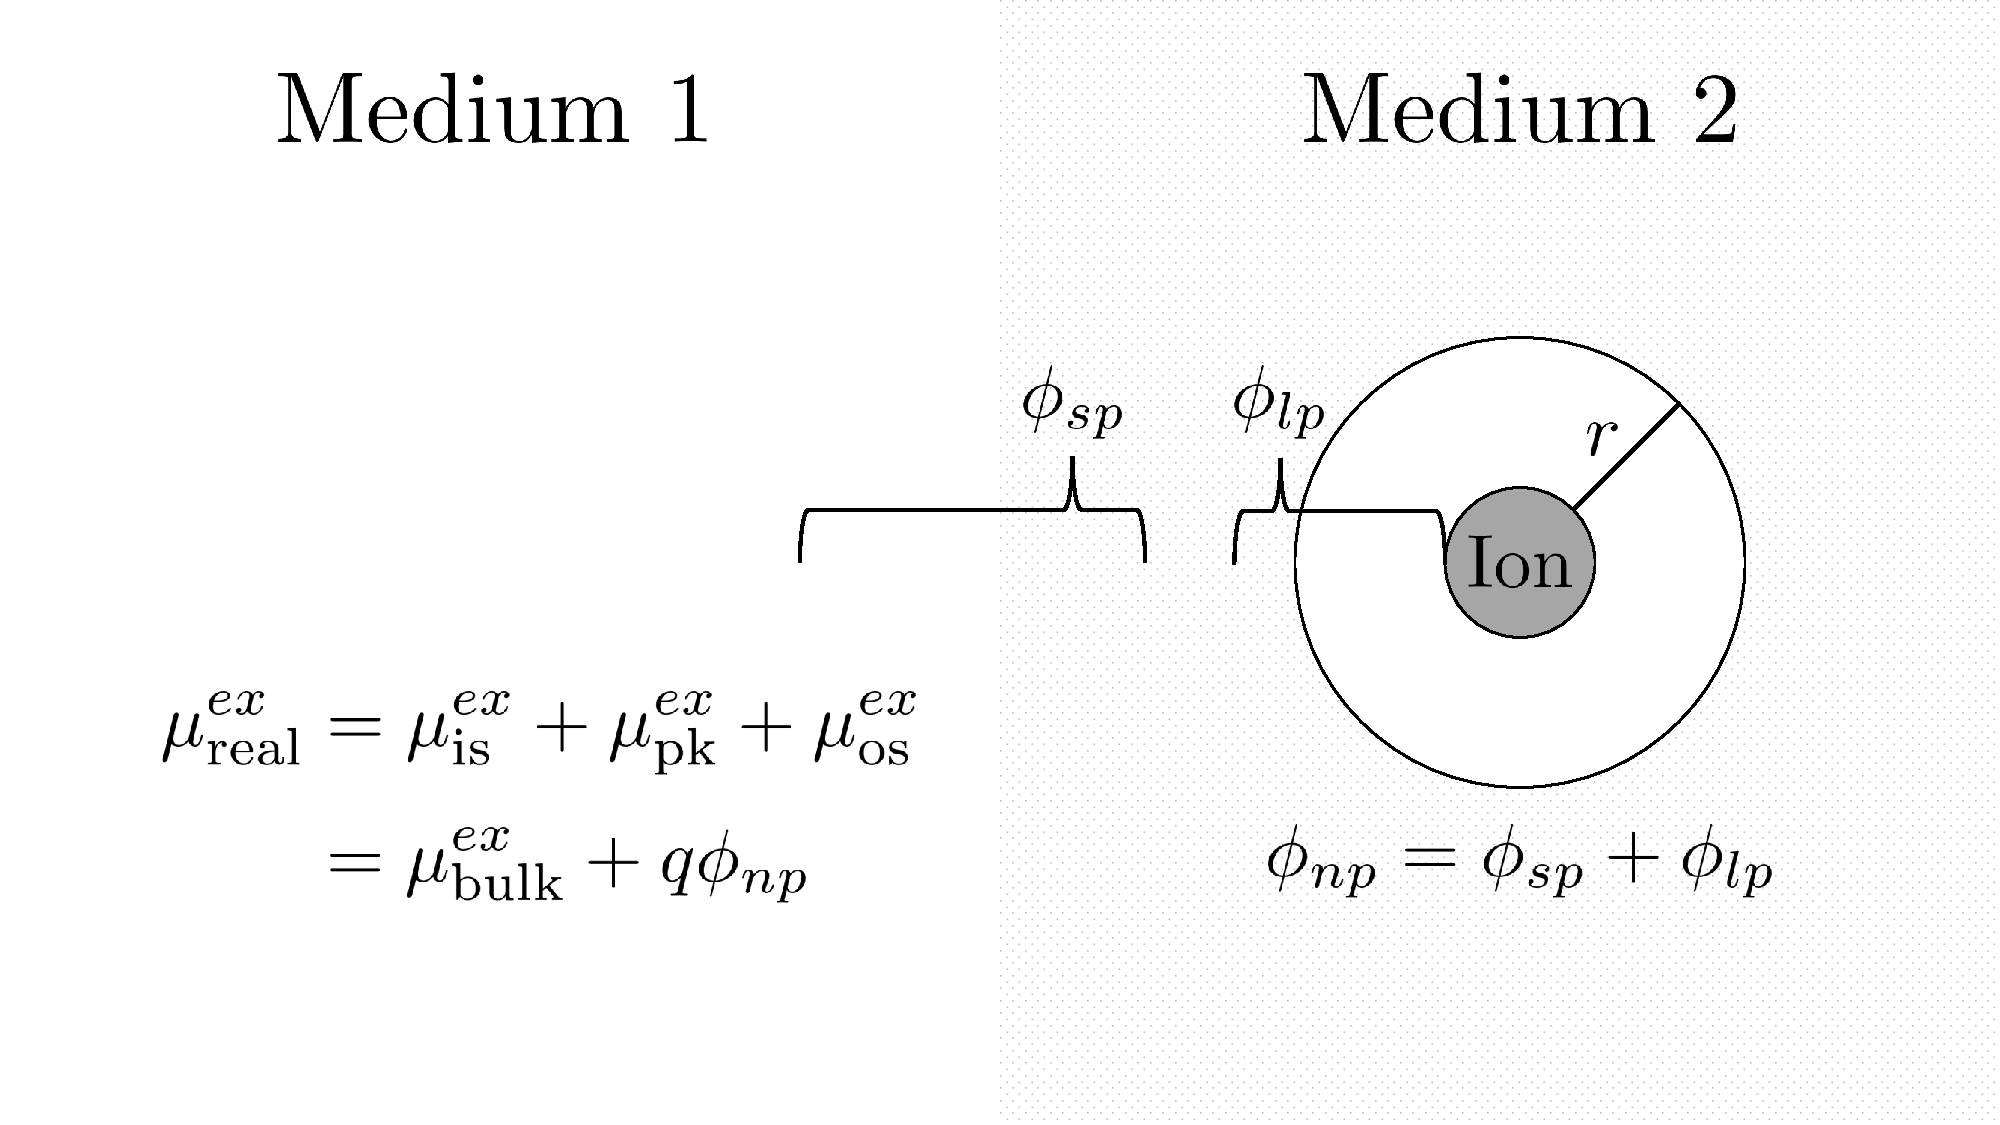
\includegraphics[width=0.98\linewidth]{images/qct_sp.pdf}
  \caption[Illustration of interfacial potentials]{Figure showing interfacial potential contributions across two distinct media to single-ion solvation free energy with 
  quasichemical partitioning. The net and local potentials can be measured as the average electrostatic potential felt by the ion solvated in medium 2 (i.e., water) in 
  a large exclusion zone with radius \emph{r}. For these calculations, the `ion' is modeled only as a spectator to define a location for the cavity. It bears no charge 
  nor interacts with the solvent in any way other than to exclude it. If medium 1 is vacuum, the potential measured in this way is the net potential. If medium 1 is 
  excluded and medium 2 is modeled in periodic boundaries then the local potential is measured. Neither potential is considered in a consistent (or correct) way in 
  molecular modeling using classical force fields and represents a serious error.}
  \label{fig:potqct}
 \end{center} 
\end{figure}  

   Point charge models yield results similar to electrochemical measurements, though there is no such simple explanation of why that is exactly. It is interesting to 
   note that applying a Gaussian smearing function to a point charge model has been seen to somewhat increase the measured surface potential suggesting that the 
   distribution of charge over all space may be important to correctly modeling surface chemistry\cite{pratt1988gaussian_sp}. Estimates of $\phi\sous{np}$ from classical 
   charge distributions or quantum estimates are very nearly identical though the magnitudes of $\phi\sous{sp}$ and $\phi\sous{lp}$ are very different and even of 
   opposite sign\cite{leung2009sp_mag,beck2013sp,remsing2014lp,warren2007hydration}. 
   
   The similarity between the surface potentials measured by electrochemical probes and $\phi\sous{np}$ led me to refer to the net potential as an electrochemical 
   surface potential. This is the average potential experienced by an ion crossing the air/water boundary and it shifts the free energy and enthalpy of solvation by 
   an amount equal to q$\phi\sous{np}$, where q is the ion charge. $\phi\sous{np}$, it's been argued\cite{ayse2012}, may play a role in anion adsorption to the air/water
   interface\cite{jungwirth2002airwat,jungwirth2006airwat}. The basicity of surface waters with an isoelectric point in the neighborhood of 
   2-4\cite{buch2007surfacid,mishra2012surfacid,beattie2014surfacid}, a shift in $\mu\sursous{ex}{H\sur{+}}$ from the bulk of +5.46 kcal/mol, also reflects the influence
   of $\phi\sous{np}$ (predicted to be half as large at the surface)\cite{ayse2012,duignan2015hydronium}. Surface effects could play a role in atmospheric 
   chemistry\cite{buch2007surfacid}. This is especially true of acid-base chemistry where the interface has been found to increase dissociation of carbonic acid
   relative to the bulk\cite{galib2014oceanacid,galib2014hbondingcarbonic} while it was noted by Baer et al. that both HCl and HNO\sous{3} are more likely to remain
   undissociated at the interface\cite{baer2014investigation}. In follow-up work, the authors found that HNO\sous{3} was about 20\% less dissociated in the interfacial 
   layers than in bulk solution even in nearly 8 M solutions\cite{lewis2011does}.

   H\"{u}nenberger and Reif\cite{hunenberger2011sp} have argued +0.13 V, the average of literature values, a reasonable estimate of $\phi\sous{np}$, which
   I contest is actually a composite of estimates of various $\phi\sous{np}$'s and $\phi\sous{sp}$'s and so the average has no physical meaning. However, this figure was
   recently adopted into a continuum model of ion solvation\cite{duignan2014ion} and to addressing the surface activity of the hydronium (H\sous{3}O\sur{+}) and hydroxide (OH\sur{-}) 
   ions\cite{duignan2015hydronium}. The free energies reported by Duignan et al.\cite{duignan2015hydronium} were observed to be particularly sensitive to the ion radius 
   used with the COSMO solvation model. An initial set of parameters produced a free energy (which includes the effect of the surface potential in the electrostatic term, 
   see Eqn. 8, of -167.5 k\sous{B}T for H\sous{3}O\sur{+} and -194.9 k\sous{B}T for OH\sur{-} at 293.15 K. In a second set, the ion radius was fit to reproduce
   experimental values with the proper standard state correction\cite{camaioni2005stdstcorr}. The radius of H\sous{3}O\sur{+} is decreased while OH\sur{-} is increased.
   The corrections adjust the electrostatic part of the free energy and reproduce the expected -189.2 k\sous{B}T and -179.4 k\sous{B}T hydration free energies for H\sous{3}O\sur{+} 
   and OH\sur{-}, respectively\cite{camaioni2005stdstcorr}. 

   The authors have adjusted the ion size to make up for what they attributed to errors in computing the ion-dependent part of the free energy but an 
   alternative explanation is that they've used the wrong surface potential. The shifts in the free energies reported by Duignan et al. are similar to the difference
   between H\"{u}nenberger and Reif's average value and the one I calculate in Chapter \ref{ch5:sec0:level1}. The charge dependent correction is another clue
   that the surface potential may be involved. But the point of this exercise is very simple: using the wrong surface potential can lead to an incorrect
   interpretation of ion solvation where interfacial effects are expected to be important. See also batteries and supercapacitors where performance is linked
   with the partitioning of ions between solid electrodes and some media (can be gas, water, organic solvent, or solid)\cite{li2015solid,schutter2015toward}.

  \section{\label{ch1:sec5:level1}Ion solvation in energy storage cyclic carbonate solvents}
   Non-aqueous environments provide a similar challenge, though there have been far fewer experiments conducted than in water. The scope of this discussion will
   be limited to carbonate solvents used in modern energy storage devices such as the Li-ion battery and supercapacitors, see Ref. \cite{goodenough2013li} for a 
   wonderful review of Li-ion technology and advancements over the years. 
   
   The Li-ion battery (LIB) is found in virtually all mobile devices (e.g., cell phones, laptops, tablets, etc.). They are also used in hybrid or all-electric 
   vehicles and have been used to power and warm our most intrepid explorers (i.e., the Mars rovers)\cite{ratnakumar2006li}. The Li-ion battery cell is composed 
   of an anode, cathode, electrolyte, and a separator. The anode is typically a carbon-based material like graphite, the cathode is a lithium metal oxide, and the
   electrolyte is a non-aqueous aprotic solvent\cite{voelker2014trace}. The separator is permeable to Li-ions and keeps the two electrodes from making contact. 
   Charging the cell with an externally supplied voltage (i.e., plugging in your device) pushes Li-ions and electrons from the cathode to the anode (electrons flow
   through an external circuit). These particles migrate back to the cathode when discharging. 
   
   Repeated cycling between charging and discharging leads to performance degradation over time through a series of chemical and/or thermal pathways. These 
   include oxidation of the electrolyte by the cathode, reduction of the electrolyte by the anode, and thermal decomposition of the electrolyte or electrodes\cite{voelker2014trace}. 
   However, some initial decomposition of the electrolyte is desired. This forms an ion permeable but nonconducting film at the electrolyte/electrode interface which
   prevents further decomposition of the electrolyte (called the solid/electrolyte interphase, SEI). Over time, the oxidative and reductive stresses of discharging
   and recharging lead to additional degradation products which not only affect battery performance but also introduce a number of safety concerns. These issues are 
   borne out of the fact that carbonate solvents have very low flash points compared to their expected operating temperature. The battery also requires a regularizing 
   mechanism to ensure the output falls between a finely specified range appropriate for the application and especially avoids overcharging (voltages greater 
   than 4.2 V)\cite{ohsaki2005overcharge,ratnakumar2006li}. Exceeding this voltage leads to rapid decomposition of the electrolyte, breakdown of the protective film, 
   evolution of CO\sous{2} at high pressure, and thermal instability resulting in irreversible damage to the cell\cite{voelker2014trace}.
   
   Suggested areas of improvement to the Li-ion battery design are delineated in a recent article by Brown et al.\cite{brown2015ion}. They are ``1) finding 
   electrodes that provide the highest energy densities, 2) developing an optimized electrolyte with the high ionic conductivity and stability at high 
   potential/temperature and 3) the appropriate solid electrode/electrolyte interphase (SEI).'' These improvements address safety concerns, capacity issues,
   small voltage range, relatively rapid degradation (even if the cell is never used), and lengthy recharge times which have limited the adoption of Li-ion 
   technology in the electrification of automobiles and other transport vehicles. The greater energy demands of the future (primarily from non-OECD countries) 
   also place a great emphasis on evolving the modern battery\cite{eia}. As does the use of storage technologies to supplement fluctuations in the output of a
   global energy grid increasingly reliant on renewable energy sources.
   
   Much of the focus to date has been on improving the materials of the cathode and anode to push the chemical potentials as far apart as possible, though under the
   new conditions the electrolyte is likely to become the bottleneck to further improvements\cite{husch2015large}. Computational screening has proven a useful tool 
   in screening potential electrolytes to limit the chemical space necessary to explore further with experiment. This reduces both cost and time of 
   development\cite{husch2015large,korth2015,schutter2015toward}. However, screening efforts thus far have focused on a number of simple to compute properties
   which makes use of continuum solvation models for the measurement of solvation free energies (a crucial factor in determining the effectiveness of an electrolyte 
   for shuttling ions between the electrodes\cite{xu2010differentiating,xu2012li}). The resulting free energies lack appropriate handling of the first solvation shell 
   and the surface potential of the solvent -- each critical to the accurate assessment of ion transport in these solvents. Additionally, it has been discussed in the
   literature that additives can greatly influence the cycling efficiency of the cell even at part per million concentrations, including in low temperature 
   conditions\cite{aurbach1992behaviour,zhang2002effect}. This reduces the relevance of studying bulk solvation properties in pure solvents as secondary and tertiary
   solvent effects are likely to significantly affect ion transport and SIE properties\cite{aurbach1992behaviour}. 
   
   It is also believed that the coordination structure around the Li\sur{+} is essential to the formation and structure of the SEI\cite{smith2014x}, though this is still
   poorly understood even in existing carbonate-based electrolytes. Thermodynamic data is almost non-existent in these solvents as well. Despite it being generally accepted 
   that both ethylene (EC) and propylene (PC) carbonate solvents tetrahedrally solvate the Li\sur{+}, there is no consensus in the literature on this point. Most experimental 
   and theoretical predictions place the coordination number in the neighborhood of \emph{n} = 4--5, with Raman intensity experiments and theoretical predictions on the lower 
   end of that range\cite{allen2014combined,bhatt2010interaction,bhatt2012density,borodin2006litfsi,borodin2009quantum,ganesh2011accurate,hyodo1989raman1,hyodo1989raman2,leung2010liion,li1999theoretical,morita1998raman,nie2013role,soetens1998molecular,takeuchi2009ion}
   while X-ray absorption, neutron scattering, and conductivity data predict 4.5 PC molecules to each Li\sur{+}\cite{kameda2007solvation,kondo2000conductivity,smith2014x}. 
   Smith et al. found that a classical polarizable force field underestimated (the same one used in Refs. \cite{borodin2006litfsi,borodin2009quantum}) the coordination 
   number relative to experiment\cite{smith2014x}. Bogle et al. found the coordination number in EC to be as high as 5.69\cite{bogle2013understanding}. The largest value yet
   was determined by Castriota et al. who estimated a Li/EC coordination number of $\sim$7 in 1 M solutions of LiClO\sous{4}\cite{castriota2003temperature}. My work in
   Chapter \ref{ch4:sec0:level1} also makes an estimate of the coordination number from density functional based simulation.
   
   A universal coordination number of 4 was assumed in the computational part of a recent study by Brown et al. which predicted the differences in binding energy between 
   Li\sur{+}-1s and Cl-2p\sous{3/2} (in ClO\sursous{-}{4}) core states in ethylene carbonate, dimethyl carbonate, (3:1) dimethyl carbonate to ethylene carbonate mixtures, 
   and dimethyl sulfoxide\cite{brown2015ion}. A comparison with near ambient pressure photoemission with liquid jet X-ray spectroscopy established that ethylene carbonate 
   more strongly solvates Li\sur{+} than the other carbonates\cite{brown2015ion}. This finding is consistent with a study by Yang et al. which established that \sur{13}C 
   chemical shifts of EC were more strongly shifted upon complexation with Li\sur{+} than other carbonate solvents\cite{yang2010investigation}. A similar conclusion was drawn 
   for the binding of EC relative to PC\cite{aurbach1992behaviour}. This strong binding contrasts with the weaker binding of anions such as ClO\sursous{-}{4} and PF\sursous{-}{6} 
   which are common constituents in commercial Li-ion batteries. 
   
   Recent efforts have also addressed whether the coordination number is shifted due to ion pairing or dissolution in the vein of the law of matching water affinities. 
   Whether ion-pairing exists in these solvents has been the subject of much debate\cite{smith2014x}. A recent pair of experimental assessments of the free energy, enthalpy, 
   and entropy of solution of KX salts, where X = (F\sur{-}, Cl\sur{-}, Br\sur{-}, I\sur{-}, NO\sursous{-}{3}, ClO\sursous{-}{4}, and SCN\sur{-}), in EC and PC were performed 
   by Peruzzi et al.\cite{peruzzi2012hofmeister,peruzzi2015solvation}. They make some attempt to connect their observations to the ``volcano'' plot I showed in Figure
   \ref{fig:collinsvolcano}. The authors note that the entropies of solution reverse sign between the two solvents despite their very similar coordination structures. This
   can only be chalked up to an anion effect which affects the EC structure more than the PC structure due to the symmetry of the molecule\cite{jones2009thermodynamic}. 
   KI was the only salt to give a negative entropy of solution in each solvent, but exhibited a terrible fit relative to the other pairs in EC which may account for this
   observation\cite{peruzzi2012hofmeister,peruzzi2015solvation}. Given the lattice energy, the enthalpy of solvation for the ion pair could be estimated. KI was also the
   only ion pair whose dissolution was exothermic in both solutions, though it was less negative in PC (though again this may reflect some error in EC). LiF, KF, KCl, and 
   KBr dissolutions are all very endothermic and larger in EC than in PC\cite{jones2009thermodynamic,peruzzi2012hofmeister,peruzzi2015solvation}. The other pairs are also
   endothermic but are more positive in PC than in EC. This has led to some discussion of a primitive kosmotrope v. chaotrope scale in the solvents\cite{peruzzi2012hofmeister,peruzzi2015solvation}.
   Since there are fewer overall sign changes in the properties of the salts it is difficult to assign kosmo/chaotropic character to the ions. Peruzzi et al. in their EC 
   paper established a single-ion scale for the potassium salts. K\sur{+} was found to be more strongly solvated than even F\sur{-}. The ``volcano'' plot the authors 
   drew from their data recovered only one slope and had no obvious kosmotrope/chaotrope cutoff as compared to water. 
   
   Attempts by Arslanargin et al. to reproduce this single-ion scale in simulation met with mixed success\cite{ayse2016ecpc}. Symmetry adapted perturbation theory calculations 
   which dissect parts of the interaction energy into chemically and physically interesting pieces (a more thorough discussion is given in Chapter \ref{ch2:sec2:level1}) 
   predicted that polarization was essential for accurate modeling of ion/EC and ion/PC complexes (even the anions). The authors also found many-body dispersion effects
   to play a role comparable to that of induction for the anions which interact with the diffuse positively charged back-end of these molecules\cite{ayse2016ecpc}. Their
   thermodynamic results for a standard force field fall short of the experimental results of Peruzzi et al.\cite{peruzzi2012hofmeister,peruzzi2015solvation}. After re-fitting
   the force field to reproduce an \emph{ab initio} binding energy curve of the ion/solvent dimer, their results overestimated those from the same experiments. The local
   potentials (-0.15 V in EC and -0.08 V in PC) were subtracted from the simulation result to establish a bulk single-ion scale in each solvent, though it is noted for pair 
   values this distinction does not matter. Thus, while these classical models may be able to appropriately mimic the dielectric behavior of pure EC and PC\cite{you2015dielectric},
   the models are simply too inflexible to exhibit an appropriate response when polarized by a nearby ion. In fact, the improvements in dielectric properties came at the
   expense of lowering the dipole of the EC and PC molecules\cite{you2015dielectric}!
   
   It was hypothesized that a proper description of polarization (not simply a universal scaling of charges to adjust the dipole) would bring the solvation free energies,
   enthalpies, and entropies into better agreement with experiment by improving the accuracy of the ion/solvent interaction part (enthalpy) and the solvent reorganization
   term (enthalpy and entropy, cancelling in free energy). The solvent reorganization term is expected to become more positive as the first solvation shell around cations
   points 4--5 large dipoles towards a central point, a clearly repulsive contribution. 
   
   My work in Chapter \ref{ch4:sec0:level1} also aims to test this hypothesis through determination of the dipole moment of molecules in the first solvation shell versus the 
   bulk. The induced dipole depends on the polarizability through a simple relation, $\vec{\mu} = \alpha\vec{E}$, where $\vec{\mu}$ is the induced dipole, $\alpha$ the molecular
   polarizability (a rank 2 tensor), and $\vec{E}$ the field. The polarizability of EC is 6.8 \AA\sur{3} and PC is 8.7 \AA\sur{3}. Compare this with water which is 1.42 \AA\sur{3}. 
   As I showed above, the polarizability is responsive to changes in molecular geometry. So they very well may be slightly larger than this around strongly polarizing cations. 
   This work is not yet ready for publication and future studies will be discussed.
   
  \section{\label{ch1:sec6:level1}Bringing it all together}
   I have presented a lot of information in this introductory section, so how best to summarize it? Ion solvation is a fundamental problem with far-reaching consequences
   in biological, industrial, atmospheric, and oceanic fields. Simple electrostatic theories exist to summarize and rationalize the behavior of salts in solution, though
   these are far from complete and often inaccurate at relevant concentrations. This is because they neglect some of the important details I discussed were essential to the
   prediction of single-ion solvation free energies: 1) ion/solvent interactions and 2) cavity formation, the reorganization of solvent around the ion. I discussed that 
   single-ion free energies in particular were essential to developing a quantitative and predictive model of ion solvation. Modern continuum theories supplement these 
   older models with non-electrostatic interactions such as polarization and dispersion through quantum chemistry, increasing their accuracy of contribution 1) and they make 
   an attempt to approximate 2). While these models are most certainly improvements over the originals, the granularity of an all-atom model is required to handle the most
   important parts of 1) and 2) which arise from the 1\sur{st} and 2\sur{nd} solvation shells. Chemical interfaces also contribute to the single-ion free energies and this
   surface potential has two contributions, at least one of which is present in \emph{all} simulations with ions. Recalling that the single-ion free energy is $\mu\sur{ex} 
   = \mu\sursous{ex}{b} + q\phi\sous{np}$, then my thesis can be broken down of as follows:
   
   \begin{itemize}
       \item Chapters 3 \& 4 -- Focus on interactions
        \begin{itemize}
            \item How can we solve $\mu\sursous{ex}{b}$ more accurately? 
            \item What level of theory is necessary?
        \end{itemize}
       \item Chapter 5 -- Focus on surface potential
        \begin{itemize}
            \item What is the value of $q\phi\sous{np}$? 
            \item Does it relate two existing thermodynamic scales?
        \end{itemize}
       \item Chapter 6 -- Focus on surface potential
        \begin{itemize}
            \item $q\phi\sous{np}$ is $q\phi\sous{sp}$ + $q\phi\sous{lp}$
            \item I demonstrate that $q\phi\sous{lp}$ contributes in periodic boundaries
        \end{itemize}
   \end{itemize}
   
\end{intro}
